\documentclass[11pt,a4paper,openany]{report}
\usepackage[utf8]{inputenc}
\usepackage[english]{babel}
\usepackage[T1]{fontenc}
\usepackage{amsmath}
\usepackage{amsfonts}
\usepackage{amssymb}
\usepackage{makeidx}
\usepackage{graphicx}
\usepackage{float}
\usepackage{lmodern}
\usepackage[dvipsnames]{xcolor}
\usepackage{tikz}
\usetikzlibrary{intersections}
\usepackage{pgfplots}
\usetikzlibrary{calc}
\usepackage{geometry}
\geometry{hmargin=2cm,vmargin=2cm}
\usepackage{fancybox}
\usepackage{mathtools}
\usepackage{enumitem}
\usepackage{tcolorbox}
\usepackage{colortbl}
\usepackage{fancybox}
\tcbuselibrary{most}
\usepackage{pifont}
\usepackage[skip = 2pt, font = footnotesize, labelfont = bf]{caption}
\usepackage{subcaption}
\usepackage{eso-pic}
\usepackage{nicematrix}
\usepackage{multicol}
\usepackage{booktabs}
\usepackage{svg}
\usepackage{derivative}
\usepackage{wrapfig}
\usepackage{stmaryrd}
\usepackage{yfonts}
\usepackage{array}
\usepackage{csquotes}
\usepackage[style=phys , backend=biber]{biblatex}
\addbibresource{bibliography.bib}
\author{Andrea}
\setlength{\columnsep}{.5cm}
\usepackage{titlesec}

% use Roman numerals for sections
\renewcommand{\thesection}{\Roman{section}}

% use Arabic numerals for subsections
\renewcommand{\thesubsection}{\arabic{subsection}}

% use letters for subsubsections with a parenthesis
\renewcommand{\thesubsubsection}{\alph{subsubsection})}

% put a period and space after numbers
\titlelabel{\thetitle\thickspace}

% Make section titles centered and bold
\titleformat*{\section}{\centering\bfseries}

% Make subsections centered and italc
 % Make subsubsections centered
\titleformat*{\subsubsection}{\centering}
\titleclass{\chapter}{straight}
\titleformat{\chapter}[frame]
{\normalfont}
{\filright
\footnotesize
\enspace \texttt{CHAPTER \thechapter} \enspace}
{8pt}
{\Large\bfseries\filcenter}

\titlespacing*{\chapter}{0pt}{10pt}{10pt}
\titlespacing{\section}{0pt}{*3}{*3}
\titlespacing{\subsection}{0pt}{*1.5}{*1.5}
\titlespacing{\subsubsection}{0pt}{*4}{*1.5}


\usepackage{amsmath}
\colorlet{shadecolor}{cyan!15}
\usepackage{fancyhdr}
\usepackage{etoolbox}
\usepackage[export]{adjustbox}
\usepackage{fourier-orns}
\usepackage{lettrine}
\usepackage{physics}
\usepackage{hyperref}
\hypersetup{
    colorlinks=false,
    linkbordercolor = {white},
    menubordercolor = {white},
    citebordercolor = {black},
    urlbordercolor = {black},
}
\captionsetup{singlelinecheck=off}

\definecolor{RoyalRed}{RGB}{157,16, 45}
\usepackage{lipsum}
\pgfmathdeclarefunction{gauss}{2}{%
  \pgfmathparse{1/(#2*sqrt(2*pi))*exp(-((x-#1)^2)/(2*#2^2))}%
}
\usetikzlibrary{decorations.markings}
\renewcommand{\headrule}{%
\vspace{6pt}\hrulefill
\raisebox{0pt}{\quad\decofourleft\decotwo\decofourright\quad}\hrulefill}
\pagestyle{fancy}
\fancyhf{}
\rhead{ \textcolor{black}{\footnotesize \today}}
\lhead{ENS}
\chead{ \textcolor{black}{· \emph{\leftmark} ·}}
\rfoot{Andrea Combette}
\fancyfoot[C]{\thepage}

\newlength{\tabcont}

\setlength{\parindent}{0.0in}
\setlength{\parskip}{0.05in}

\setcounter{tocdepth}{4}
\setcounter{secnumdepth}{4}

\begin{document}
\begin{titlepage}
    \AddToShipoutPictureBG*{
        \begin{tikzpicture}[overlay,remember picture]
            \draw [line width=3pt]
            ($ (current page.north west) + (2cm,-2.0cm) $)
            rectangle
            ($ (current page.south east) + (-2cm,1.8cm) $);
            \draw [line width=1pt]
            ($ (current page.north west) + (2.15cm,-2.15cm) $)
            rectangle
            ($ (current page.south east) + (-2.15cm,1.95cm) $);
        \end{tikzpicture}
    }
    \begin{center}
        \vspace*{2cm}
        \emph{\footnotesize{Department of physics, École Normale Supérieure, Paris}}

        \emph{\footnotesize{Swiss Plasma Center, EPFL, Lausanne}}


        \vspace*{1cm}

        \textsc{Trapped Electron Mode}

        \textsc{Characterization by Short Pulse Reflectometry}
        \vspace*{1cm}

        \rule{14cm}{2pt}\vspace{.7cm}

        \Large{\textbf{Master Thesis 2024}}

        \vspace{.5cm}
        \rule{14cm}{2pt}
        \vspace{1cm}

        \Large Andrea Combette

        \vspace{3cm}

        \raisebox{-5pt}{\quad\decofourleft\decotwo\decofourright\quad}

        \vspace{2cm}
        \vspace{1cm}

        \begin{minipage}{14cm}
            \small{\textbf{Supervisors:}}
            \vspace{.5cm}

            \small{\textbf{Dr. Oleg Krutkin \null\hfill Pr. Jean François Allemand}}

        \end{minipage}
        \vspace{2cm}


        % \begin{minipage}{14cm}
        %     \small{
        %         \textbf{Cautionary note : } This paper is a report on numerical methods for the shallow water equations and gravity waves. It is not intended to be a complete and rigorous study of the subject. The reader is invited to refer to the references for further details.
        %         It has been made by a Master Student, with some background in physics and mathematics, but no prior knowledge of the subject. It is therefore not intended to be a reference for experts in the field.}
        % \end{minipage}

    \end{center}

\end{titlepage}

\newpage
\begin{multicols}{2}
    \tableofcontents

\end{multicols}
\newpage


\begin{center}
    \textbf{ABSTRACT}
\end{center}
\fontsize{9}{10}\selectfont

\lettrine[loversize=.30,findent=.21em,nindent=2.5pt]{\color{black} O}{ne} \emph{of the common goals in experimental magnetically confined fusion research is characterization of the plasma turbulence. To that end, TCV tokamak features a novel short-pulse reflectometry (SPR) diagnostic, which can potentially be utilized to measure properties of the turbulence.
    It is essentially a radar system, where the plasma is probed by a short (under ns) microwave pulse in the presence of the cut-off (reflection) area from which the pulse reflects back into the probing antenna. The position of the cut-off for a particular probing frequency (50-75 GHz) range is determined by the plasma electron density. Thus, by measuring the delay between probing and reflected pulse corresponding to different probing frequencies, the information about the electron density profile is inferred including its turbulent perturbations.
    Unfortunately, the complex interaction of microwaves with magnetized plasma makes it difficult to establish the connection between SPR measurements and properties of the turbulence. Numerical modeling utilizing the synthetic diagnostic approach was carried out to establish this connection for the case of low turbulence amplitudes (linear regime). However, the case of large turbulence amplitudes (nonlinear regime) is yet to be explored.
    Within the project a systematic analysis of the SPR diagnostic in the nonlinear regime will be carried out. The numerical finite difference code CUWA, which solves the wave equation for a given plasma density, magnetic field and provides synthetic reflected pulse will be utilized. The main goal of the project is identifying markers that can be used to determine if the diagnostic is operating in the nonlinear regime and assessing the possibility of determining the turbulence parameters regardless.
}
\fontsize{10}{10}\selectfont

\begin{multicols}{2}
    \chapter{Theoretical Background}

    \section{Nuclear Fusion}
    \subsection{Fusion Reaction}
    \lettrine[lines=2, lhang=.3, nindent=0pt]{\color{black} T}{he} nuclear fusion reaction is the process by which two atomic nuclei combine to form a heavier nucleus. It is accompanied by the release or absorption of energy depending on the masses of the nuclei involved. Indeed, the lighter are nuclei, the  more  energy is released due to the overcoming short-range nuclear force for light nuclei.
    However, to overcome the Coulomb barrier the reactant must be sufficiently close for a long enough time to allow the quantum tunnel effect between both particles. To do so, we must heat up the reactant to huge temperatures such that these latter are ionizing and turning into plasma. We found that the probability of collision (cross section) is the best \ for the Deuterium-Tritium mix.

    \begin{align*}
        \text{D}^2 + \text{T}^3 & \rightarrow \text{He}^4 + \text{n[17.6 MeV]}
    \end{align*}
    \subsection{Tokamak confinement}
    The key component of the fusion process is how long we can confine the plasma. This confinement can be of several kinds. One of the most promising and old, is the Tokamak vessel, which uses magnetic confinement to keep the plasma in a toroidal shape. The plasma is heated up to several million degrees, and the fusion reaction can be sustained. The energy released by the fusion reaction is used to heat up the plasma, and to sustain the reaction. The energy balance is given by the Lawson criterion, which is a measure of the energy confinement time over the energy loss time.
    The energy confinement time is given by the plasma density, temperature and the energy loss time is given by the plasma losses.

    $$n \tau E \ge 1.5.10^{20}{\frac {\mathrm {s} }{\mathrm {m} ^{3}}}$$
    \begin{figure}[H]
        \centering
        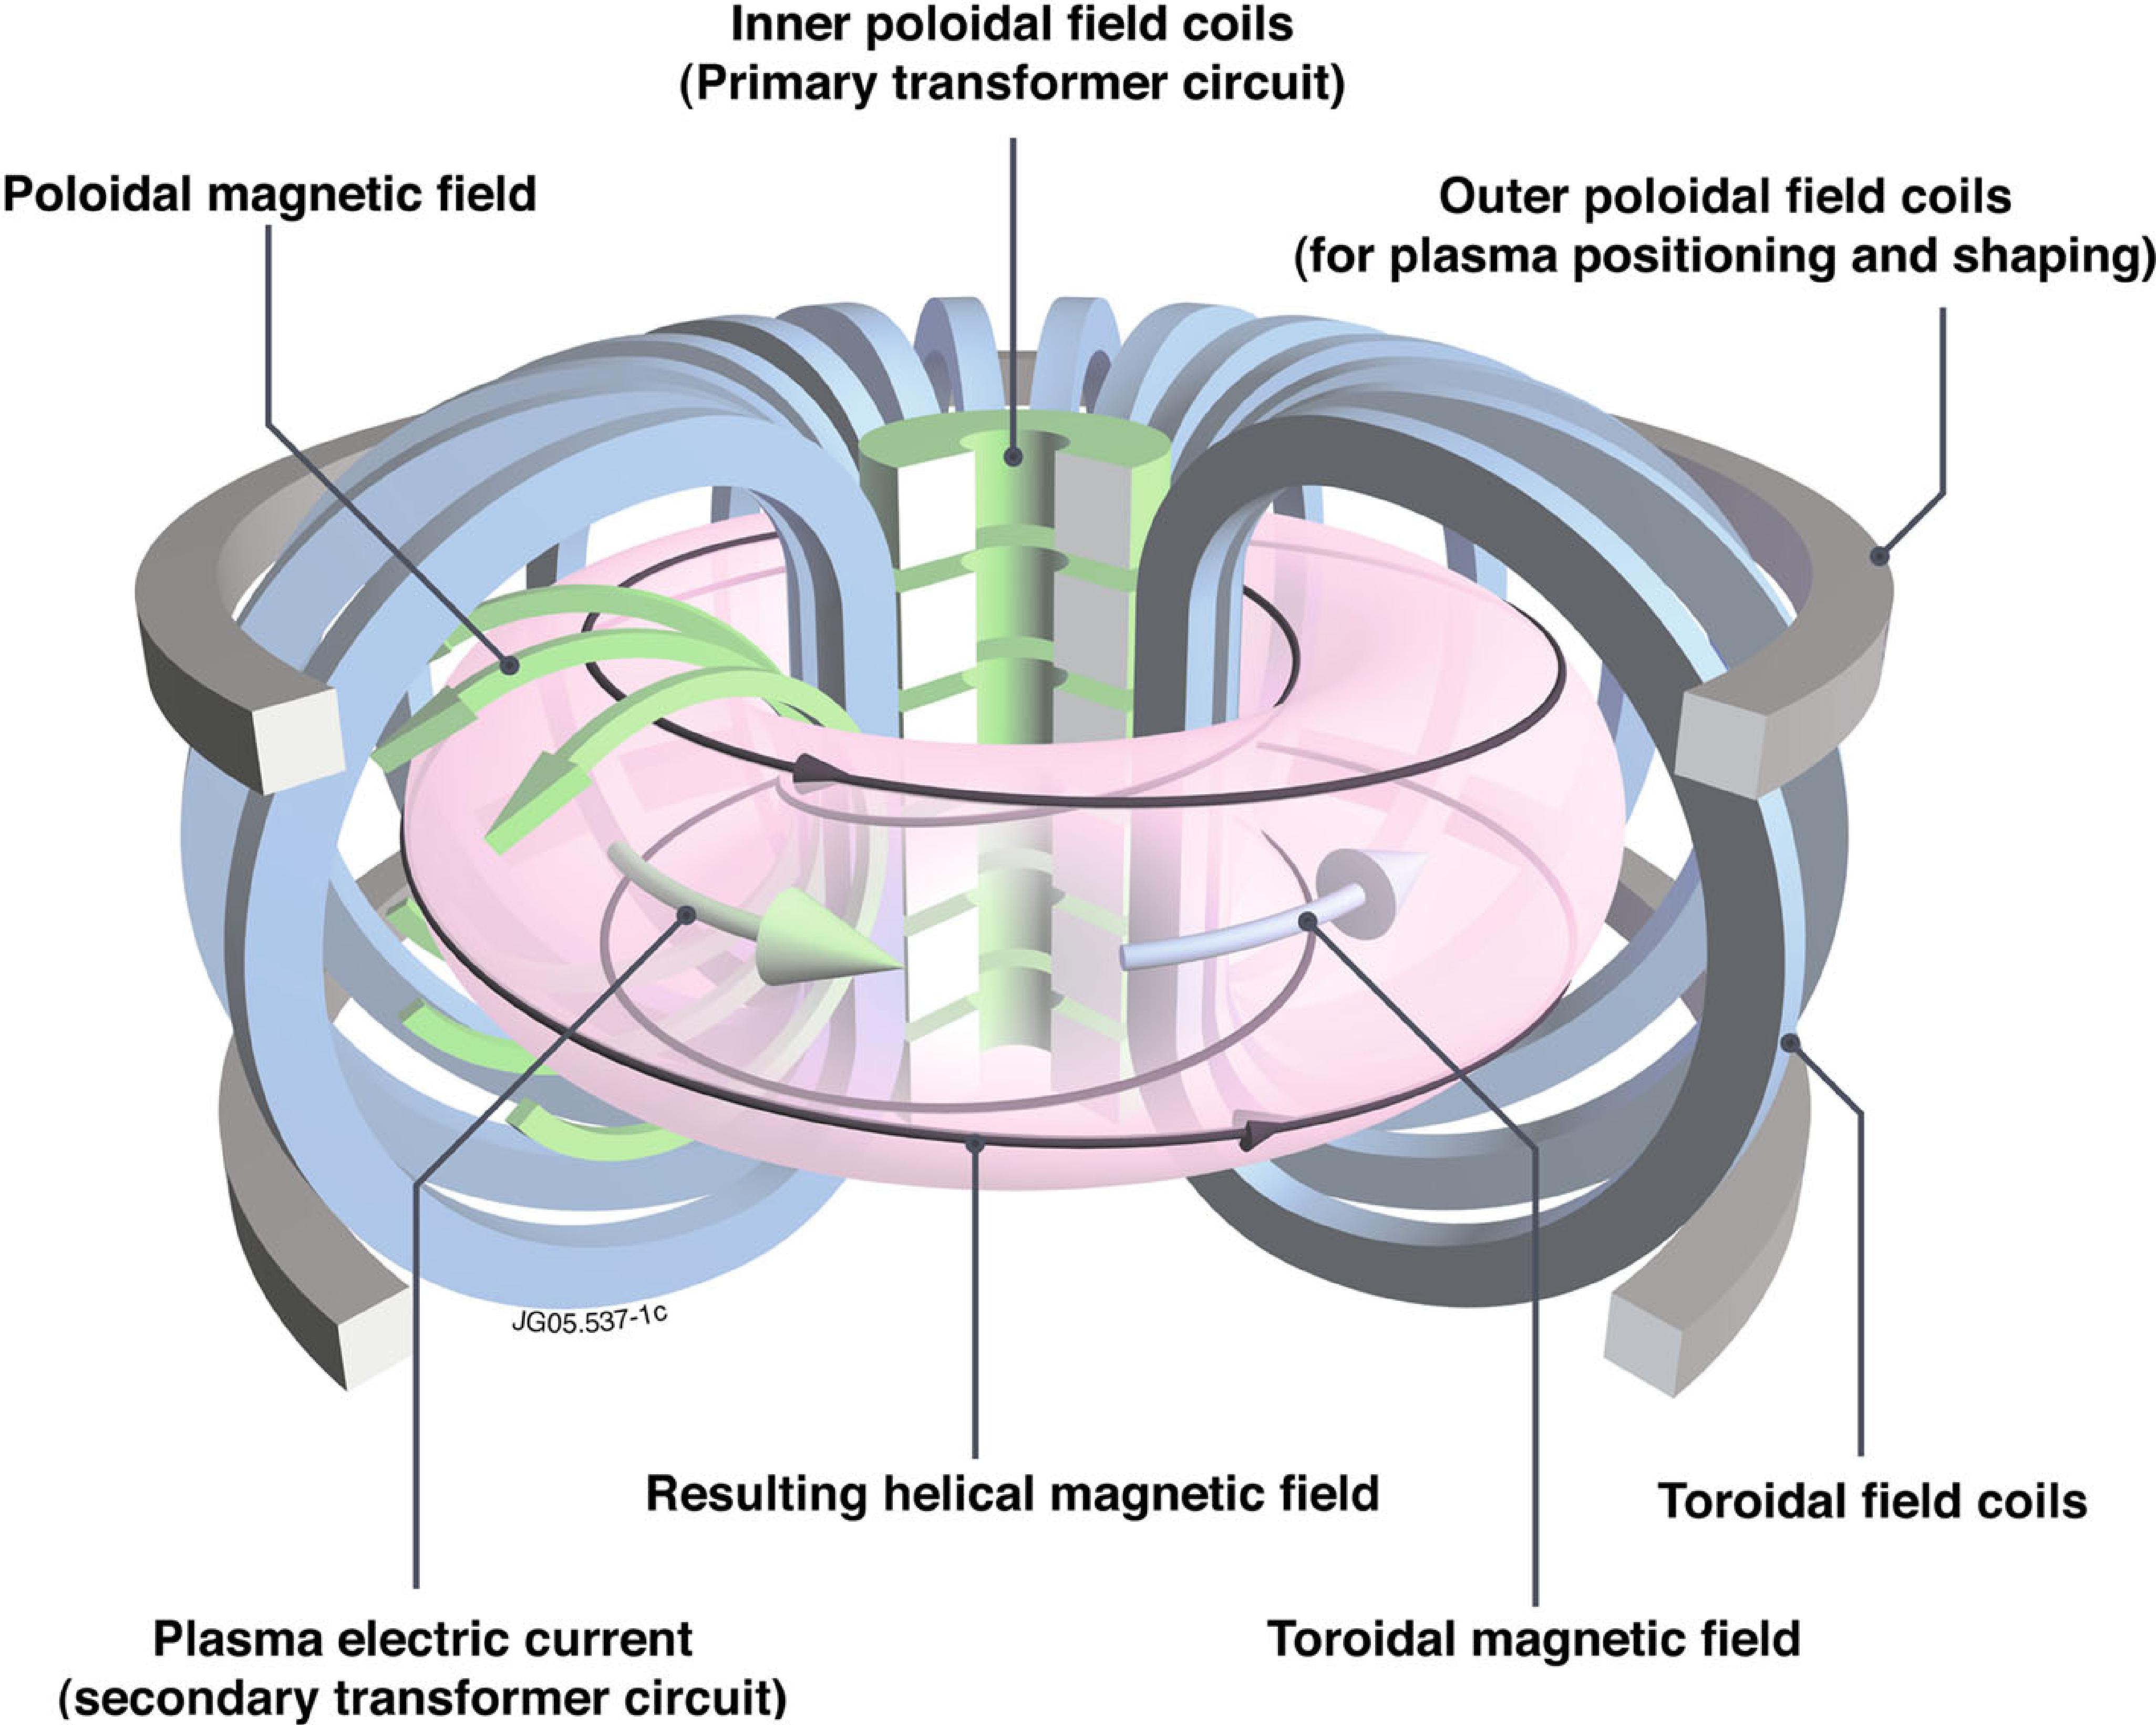
\includegraphics[width=1\linewidth]{./figures/tokamak.png}
        \caption{simplification of Tokamak device, the toroidal magnetic field is generated by the coils, and the poloidal magnetic field is generated by the plasma current and the poloidal field coils. The plasma is heated up by several device, and the fusion reaction can be sustained.}
        \label{}
    \end{figure}

    This confinement is realized by applying a strong magnetic field in the toroidal direction. The magnetic field is generated by a set of coils, which are arranged in a toroidal shape, and the plasma is heated by various method \cite{Heating}. The neoclassical geometries at stake in the tokamak leads to several physics phenomena such as charge separation in the tokamak, drifts cinematic and turbulences. The curvature and the gradient of magnetic field \cite{piel2018plasma} imposed by the geometry leads to $E \times B$ drift. Which impose to the tokamak a poloidal magnetic field component to counter this effect. This twist in the field line is called the safety factor and is defined as :
    $$q(\Psi) = \frac{1}{2\pi}\frac{\delta \chi (\Psi)}{\delta \Psi} \approx \frac{B_{tor}r}{B_{pol}R} \, ,$$
    With $\chi$ the toroidal magnetic flux. This safety factor is one of the most important measures in tokamak since the induced magnetic properties on the rational magnetic surface \footnote{Only rational value of the safety factor allows periodic field line} are of paramount importance for the confinement of the plasma. Indeed, we can define the shear stress as $\hat{s} = \frac{r}{q}\dv{q}{r},$ which measures how much the magnetic field line are twisted along the small radius of the tokamak. This shear explains why the turbulences grow on rational surfaces (no Landau Damping $k \centerdot B = 0$, \cite{TEM_landau_rational}), and how they are damped into bigger scale flow (zonal flow) see \cite{Scaling_TEM}.
    Indeed, the consideration of the magnetic surfaces is also at the foreground for solving Ballooning equations in toroidal geometry, since it will drive the definition of the toroidal functions of Ballooning modes, every discussed instabilities can be expressed using a toroidal geometry in the Ballooning space \cite{TEM_ballooning,DW_transport}. In addition to that the safety factor allows to have an insight of the strength of the toroidal current, which follows the $q$-profile (max in the center), this explains why the toroidal velocity of particle is lower on the edge than in the center, which allows some particle to be trapped in banana orbits.


    \section{Transports in Tokamak}
    Anomalous transport is a crucial subject in tokamak research, indeed it causes a huge drop of the energy confinement through a enhanced particle radial flux. Here we will study micro-instabilities, i.e small scale turbulences (gyro-bohm scaling \cite{Scaling_TEM}), whose radial transport is really high and largely controlled by low frequency modes \cite{DW_transport}. For these type of instabilities, the study is based on Kinetic Vlasov theory.
    Several types of micro-instabilities exists from \textbf{TEM} to \textbf{ITG} and \textbf{ETG} instabilities. These instabilities cause a transport of energy from the core of the plasma to the edge, where it can be evacuated, the largest transport in the TCV is due to the unstable \textbf{TEM} mode \cite{Krutkin_thesis,TEM_slow}. This mode is the results of the resonant interaction between trapped electron and Drift Wave (DW), it can be colisionless or dissipative, basically the trapped electron are transfering energy to the growing wave.
    \subsection{Trapped particles and drifts}

    There are two type of kinetic for electrons in the tokamak : run-away  or passing and trapped electrons. Majority of the electrons are passing since to be trapped electrons must verify  : $v_\parallel \ll v_{th}$ \cite{book_banana}\cite{Banana_distr_runaway}. However trapped electrons present a transit time much larger than passing one, this leads to greater interaction with the DW.
    These different of behavior regarding the DW leads to small scale instabilities.
    \subsubsection{Trapped particles}
    For a colisionless plasma $ \nu \ll w$, with $\nu$ the collision frequency and w the frequency of the considerated wave, the main radial transport is caused by particle with low parallel velocity. Indeed, when the toroidal component of the magnetic field is much larger than the poloidal component, $\vert B_\Phi \vert \gg \vert B_{pol} \vert$ we have the simple $B$ relation for a torus $$B\propto \frac{1}{R-R_0} \, , $$ then in the $(r, \theta, z)$ coordinates we have  :
    $$B = B_0\left[1 - \frac{r}{R_0}\cos(\theta)\right]$$
    Hence, taking into account the toroidal drift we can derive the following equations using the guiding center equations \cite{book_banana}:
    $$\dv{t}\left( r +\frac{m}{qB_p}v_\parallel\right) = 0 ,\, r - r_0 = -\frac{m}{qB_p}v_\parallel$$
    $r_0$ indicates the position of the turning point where the mirror effect occurs \cite{TEM_mirror_localization}. To be trapped the particle velocity should verify $v_\parallel \ll v_\perp$ more precisely from a simple energetic approach \cite{TEM_slow}$$0 \leq v_\parallel \leq \sqrt{2\epsilon} v_\perp \,.$$ This partially explains why the velocity distribution of the electron \cite{TEM_slow,Banana_distr_runaway}is modified from a Boltzmann distribution to a more complex one, leading in a drop of conductivity (Spietzer condicivity). This also explain why the \textbf{TEM} dissipative and colisionless are highly locallized in the trapped electron region. The banana shape formed has then the following width :
    $$\Delta r = \frac{m}{qB_p}v_\parallel \, $$

    This banana shape can be interpreted as a simple Lorentz force acting on the particle animated by a sufficiently high vertical drift motion.
    \begin{figure}[H]
        \centering
        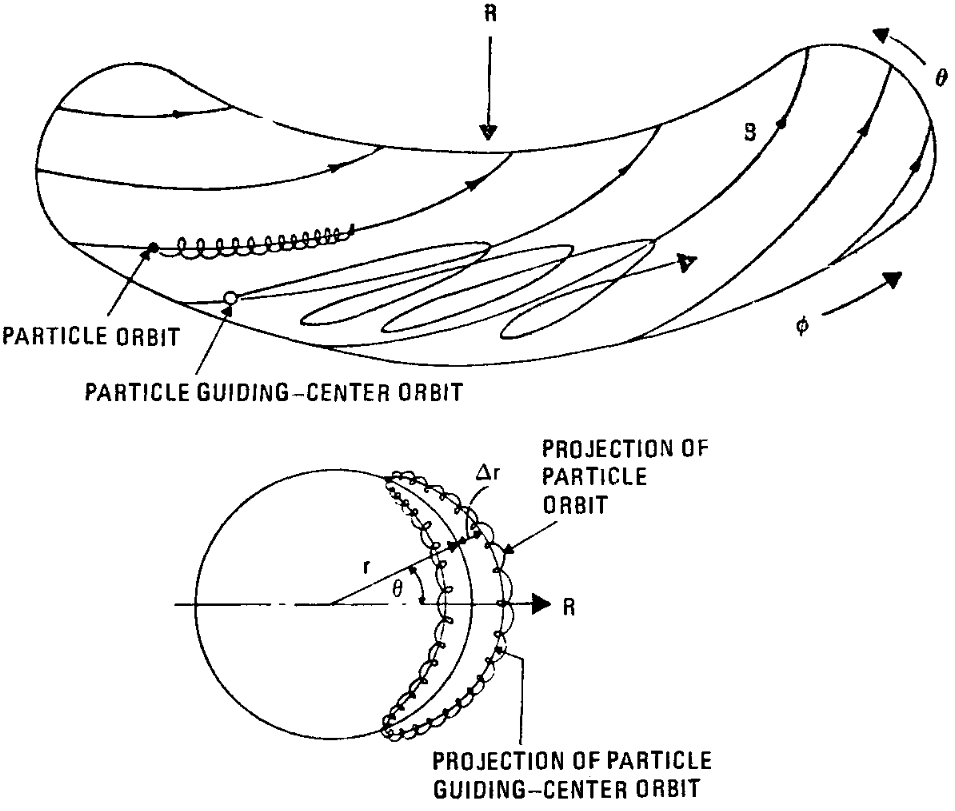
\includegraphics[width=1\linewidth]{./figures/banana.png}
        \caption{Trapped particle motion in the tokamak, the banana shape is due to the toroidal magnetic field, the particle is trapped in the magnetic well, and can interact with the DW. the second figure shows a cross section of the torus where we project the one banana orbit of the particle. From \cite{book_banana,Banana_distr_runaway}. Hence, if a wave is resonating with the particle, with a lower frequency than the transit time of the particle, the particle can exchange energy with the wave in a quasi-adiabatic way. (see after)}
        \label{}
    \end{figure}

    \subsubsection{Drift waves}
    Electron  DW instabilities that are at stakes here are governed by the famous \textbf{Hasegawa-Wakatani} \cite{Hasegawa,Wakatani} equation due to non-adiabatic response of the electrons (the equilibrium is not reached after each oscillation of the wave) derived from a simple version of the drift kinetic equation from Vlasov theory. Hence, let's remind the general form of the general form of the H-W equation~:
    \begin{equation}
        \begin{cases}
            \rho_s^2
            \dv{t}\nabla_\perp^2 \Phi= D_\parallel\nabla_\parallel^2(\tilde{\Phi} - \frac{T\tilde{n}}{|e|n_0}) \\
            \frac{1}{n_0}\dv{t}\tilde{n} + \frac{v_r}{n_0}\partial_r n_0 = D_\parallel\nabla_\parallel^2(\tilde{\Phi} - \frac{T\tilde{n}}{|e|n_0})
        \end{cases}\,.
    \end{equation}

    With $\rho_s$ the ion sound radius, $D_\parallel$\footnote{the parallel diffusion coefficient provides insights of the electrons-ions collision frequency $D_\parallel = \frac{v_{the}^2}{\nu_{ei}}$} the parallel diffusion coefficient, $\Phi$ the electrostatic potential, $\tilde{n}$ the density perturbation, $v_r$ the radial velocity, $n_0$ the equilibrium density, $T$ the electronic temperature, $e$ the electron charge.

    In the adiabtic limit \cite{Trapped_Particle_Mode}, i.e when the particles diffuse faster than the wave, we can assume a simple a Boltzmann distribution of electrons with a small perturbation :
    $$\frac{\tilde{n}}{n} \approx \frac{\vert e \vert}{T} \tilde{\Phi} + \tilde{h}$$ this finally leads to the \textbf{Hasegawa-Mima} \cite{Mima} equation under the assumption : $ v_{thi} <\frac{w}{k_\parallel} \ll v_{the}$.
    \begin{equation}
        \begin{cases}
            \rho_s^2\dv{t}\nabla_\perp^2\tilde{\Phi} \approx \frac{1}{n_0}\left(\dv{\tilde{n}}{t} + \tilde{v_r\partial_r n_0}\right) \\
            \partial_t \frac{\vert e \vert \tilde{\Phi}}{T} + \partial_t \tilde{h} - \rho_s^2\dv{t}\nabla_\perp^2\tilde{Phi}  + v^{*}\partial_y\frac{\vert e \vert \tilde{\Phi}}{T} = 0
        \end{cases}
    \end{equation}
    With $v_* = \rho_s c_s / L_n$ and $L_n$ the gradient scale of the equilibrium density $-\partial_r n_0 / n_0$. This leads to the following dispersion relation for the drift waves with $w_r$ the real frequency of the wave and $\gamma$ the growth rate (the imaginary part of the frequency) :
    $$\omega_r = \frac{w_{*}}{1 + k_\perp^2\rho_s^2}, \quad \frac{\gamma}{w_r} = \pi \frac{w_r - w_{*}}{k_\parallel v_{e,th}}$$

    We can denote $\frac{w-w_*}{k_\perp^2v_{e,th}}$ the non-Boltzmann factor for electron DW. The reader will note that this study is independant of trapped electron, this is why in order of magnitude the growth rate is quite low, however when we increase the transit time of electron (by trapping),
    we can show \cite{Sazn_diego}, that the non-Boltzmann factor is increasing, leading to a higher growth rate, notably because of the introduction of $w_{D,e}$ the electron curvature drift frequency. Indeed, for colisionless trapped electron mode the non-Boltzmann factor is given by : $\frac{w - w_*}{w_{e,D}}e^{-R/L_n}\sqrt{\frac{R}{L_n}}$ which is definitively larger than the electron DW non-Boltzmann correction factor.
    leading to the following growth rate : $$\frac{\gamma}{w_r} = i \pi \frac{w - w_*}{w_{e,D}}e^{-R/L_n}\sqrt{\frac{R}{L_n}},$$ explaining why \textbf{CTEM} are much more unstable than classical electron DW. Explaining also why the main instabilities are located in the banana region where the coherence time of the electrons are much more larger, same conclusions can be driven from the Dissipative Trapped electron mode \cite{Trapped_Particle_Mode}. This instabilities leads to inverse cascade of energy (\emph{Kolmogorov}), contributing to highly non linear interaction with mesoscale structures (zonal flow) \cite{San_diego,Krutkin_thesis,DW_transport}.
\end{multicols}

\begin{figure}[H]
    \centering
    \includegraphics[width=1\linewidth]{./figures/balloning_TEM.png}
    \caption{Cross section view of tokamak with negative shear flow - On the left we have the fourier Ballonning mode $n = 6$, characteric from the TEM mode, it presents this characteristic tilting of the wave vector $k_{\perp}$, and a radial translational symetry. On the right we have a simulated TEM mode, with the same shape structure characterics, we will note the presence of multiple modes, teared and more tilted by the zonal flow, explained by the non linear interaction between these two types of flow, reproduced from \cite{TEM_simulation,Ballooning_transform} }
    \label{}
\end{figure}
\begin{multicols}{2}
    \subsection{Radial Transport}
    These micro-instabilities are one of the best candidates to explain high radial transport, indeed as we saw previously the resonating trapped electron allows a high fluctuation in the density field and in the magnetic pressure. Indeed we can show that the radial particle flow does not vanishe (as normal), in this case with a high contributio of the resonant trapped electron to the mean transport \cite{San_diego}. This radial dependency is the only density dependency retained for the following part.

    \section{Wave propagation in plasma}
    \subsection{Plasma as a medium}
    To study the density profile, many diagnostics methods exists ,like Doppler Reflectometry, RCDR, Short pulse reflectometry \dots The study here will be based on the Short Pulse Reflectometry (\textbf{SPR}), this methdod consists in probing the magnetized plasma with a short gaussian Pulse (<ns) microwaves operating in the time domain at a fixed frequency under normal incidence with respect to the cut-off surface and the variation of the delay of the reflected pulses. The probing signal, is sensitive to density variation since it will change the cut-off position, this is why it can
    be used to have deeper insights of the turbulences characteristics
    \subsection{Wave equation}
    Assuming a monochromatic electromagnetic-wave and using the Maxwell equations, we can derive the local complex dieletric tensor, and the considerated wave wave equation :

    \begin{equation}
        \begin{rcases}
            \laplacian E -  \vec{\nabla}\nabla \cdot E = -\frac{\omega^2}{c^2} \hat{\epsilon} E \\
            \hat{\epsilon}_{ik} = \delta _{ik} - \frac{4\pi i}{\omega} \sigma_{ik}
        \end{rcases}
    \end{equation}
    with $\sigma_{ik}$ the conductivity tensor. To establish this equation multiple assumption have been made, linear Ohm's law is applicable, cold plasma (cite), neglect chaotic motion of the particles, which implies neglecting the kinetic effect. To simplify the problem we will assume the plasma to be stationnary and neglect all kinds of damping. Then in a carthesian coordinates system with $z$ axis driven by a constant magnetic field,
    $\vec{B} = B_0\vec{e}_z$, we can derive the following dielectric tensor\cite{Thomas H.Stix}
    $$\hat{\epsilon} = \begin{pmatrix}
            \epsilon & ig       & 0    \\
            -ig      & \epsilon & 0    \\
            0        & 0        & \eta
        \end{pmatrix}$$
    With : $\epsilon = 1 - \frac{\omega_{pe}^2}{\omega^2 - w_{ce}^2}$, $g = \frac{w_{ce}w_{pe}^2}{w(w^2 9 W_{ce}^2)} - \frac{w_{ci}w_{pi}^2}{w(w^2 9 W_{ci}^2)}$;
    $ \eta  = 1 - \frac{w_{pe}^2}{w^2} -  \frac{w_{pi}^2}{w^2}; \quad w_{pi} = \sqrt{\frac{4\pi n e^2}{m_i}}; \quad w_{ci} = \frac{eH}{m_i c}$

    $w_{pi}$ stands for the electron or plasma frequency and $w_{ci}$ is the cyclotron frequency for the i species. We will consider the electron component preponderant in the next study since we are dealing with microwave frequency. The wave equation can be simplified to the following :

    \begin{equation}
        \begin{rcases}
            (S_{yz} - \epsilon)E_x - igE_y - \Pi_{xy}E_z = 0 \\
            (S_{zx} - \epsilon)E_x + igE_x - \Pi_{yz}E_z = 0 \\
            (S_{xy} - \eta)E_z -\Pi_{xz}E_x - \Pi_{yz}E_y = 0
        \end{rcases}
    \end{equation}
    Defining : $S_{ij} = N_i^2 + N_j^2; \quad \Pi_{ij} = N_iN_j ; \quad N_{i} = \frac{k_iw}{c}$
    For the \textbf{SPR} study the wave is perpendicular to the external magnetic field, hence we can simplify the system to the following :
    \begin{equation}
        \begin{rcases}
            (N_y^2 - \epsilon)E_x - igE_y = 0 \\
            (N_x^2 - \epsilon)E_y + igE_x = 0 \\
            (S_{xy} - \eta)E_z = 0
        \end{rcases}
    \end{equation}

    Which leads to two different types of solution respectively the ordinary mode ($\mathcal{O}$) and the extraordinary mode ($\mathcal{X}$).
    \setlength{\tabcolsep}{18pt}
    \renewcommand{\arraystretch}{1.5}
    \begin{center}
        \begin{tabular}{|| c  | c||}
            \hline
            $\mathcal{O}$       & $\mathcal{X}$                       \\
            \hline\hline
            $S_{xy} - \eta = 0$ & $(N_y^2 - \epsilon)E_x - igE_y = 0$ \\
            $E_y = 0$           & $(N_x^2 - \epsilon)E_y + igE_x = 0$ \\
            $E_x = 0$           & $E_z = 0$                           \\
            \hline
        \end{tabular}
    \end{center}
    The $\mathcal{O}$ mode corresponds to the mode with electric field parallel to the external magnetic field, hence the propagation does not depend on this latter but only on the density profile. The $\mathcal{X}$ mode is the mThisode with electric field perpendicular to the external magnetic field, hence the propagation depends on the magnetic field and the density profile. The dispersion relation of the wave can be derived locally from the wave equation, and we can obtain :
    \begin{equation}
        k^2 = \frac{w^2}{c^2} \eta \approx \frac{w^2}{c^2}\left(1 - \frac{n}{n_c}\right); \quad n_c = \frac{m_ew}{4 \pi e^2}
        \label{eq:Dispersion_relation}
    \end{equation}

    Here we can see that the wave number vanish at $n = n_c$, this is the cut-off layer where the wave is reflected.
    The k-spectrum of the $\mathcal{X}$ is much more complicated and include plasma resonances where thermal effects must be taken into account. For this study we will limit ourself to the $\mathcal{O}$ mode. Then from solving the Helmotz equation (local dependancy of the wave number) $$\pdv[2]{E_z}{x} + k(x)E_z = 0$$ and appying the \textbf{WKB} approximation (slow variation of the plasma parameters), i.e assuming a a solution of the form $E_z = A(x) \exp(i\Phi(x))$, with $A$ varying slowly and $\Phi$ varying quickly, we can derive the following expression for the Electric field:
    $$E_z(x) = \frac{E_z}{\sqrt{\frac{c}{w}k(x)}}\exp\left(i\int_0^x k(x')dx'\right)$$
    The WKB approximation will be used in the one dimensional approach (see Chapter 2), and in the \textbf{CUWA} code for computing the ray tracing in order to adjust the size of computation Yee cells \cite{CUWA} and the computation domain.
    \section{CUWA code overiview}
    The CUWA code is a \textbf{GPU} based computations scheme with a Python-CUDA frameworks, using finite difference scheme for spatical dependancy applied to the three different fields :
    $E, B, J$ and the well-known leap-frog time stepping.It is used to simulate the propagation of electromagnetic wave inside a \textit{"cold plasma"}. The spqaial finite difference scheme is based on the FDTD Yee's method \cite{Yee}, with slight modifications.
    It solves the discrete version of the Maxwell's equations with a cold Plasma current Response $\textbf{J} $ :

    \begin{equation}
        \begin{cases}
            \pdv{t}\textbf{B}  = - \nabla \times \textbf{E}                                                 & \text{} \\
            \pdv{t}\textbf{E} = c^{2}\nabla \times \textbf{B} - \frac{\textbf{J} }{\epsilon_0 }             & \text{} \\
            \dv{t} \textbf{J} \nu \textbf{J} = \epsilon_0 w_p^2 \textbf{E} - \textbf{J} \times \textbf{w}_c & \text{} \\
        \end{cases}
        \label{eq:Maxwell}
    \end{equation}

    with $w_p$ the electron plasma frequency, $\nu$ the electro collision frequency and $w_c$ the electron cyclotron frequency. To limit the computational cost, the computation domain is amended with a convolutional perfectly matched layer (\textbf{PML}) to ensuring any reflected singals are small (well used in open boundaries systen). It can be viwed as a sponge layer for electromagnetic wave.

\end{multicols}

\begin{figure}[H]
    \centering
    \includegraphics[width=1\linewidth]{./figures/field_SPR.pdf}
    \label{}
\end{figure}
\captionof{figure}{\textbf{SPR} setup using the \emph{O.Krutkin and A.combette \textbf{LEONARDO} simulations from the \textbf{CUWA} code}, the probing wave is sent to the plasma, and the reflected wave from the cut-off is measured, the delay between the two waves is a measure of the plasma density profile, in addition to the pulse shape that has been altered by the turbulenences (eq). Here we plot the contours of the density profile, with cold density perturbations (black contour lines on the left plot), the probing wave is reflected by the cut-off layer (initial probing wave on the left and after a $\Delta t \approx 10 ns$ we got the reflected scattered wave on the right). The third plot on the right shows the density profile width its perturbations (filled), a liner density profile $$n(x,y) = \frac{x}{L} \left(n_c + \delta n(x,y)\right).$$ as been chosen accoriding to (cite). Note that this linear correction made on the amplitude of the turbulence fields, follows from the non-adiabatic perturbations \cite{San_diego}, and his more relevant than a simple constant amplitude turbulence field. The curvature of the grid has been set to the $R = 0.25m$ to mimic the TCV geometry.}
\begin{multicols}{2}
    \chapter{Linear Regime Study}
    The goal of this study is to find a way to link the plasma density perturbations to the reflected pulse characterics. First we will study a simple 1 dimensional model proposed by (\emph{Oleg Krutkin}) applied in a given range of turbulence amplitude and size and then we will extend this study to a morte general 2D model using the \textbf{CUWA} code.
    \section{1 dimensional study}
    Assuming a simple plasma density profile $n(x)$, we can study the wave propagation in the plasma. The goal of this approach is to find a way to link the plasma density perturbations to the reflected pulse delay. To retrieve some information about the pulse delay we will
    use a statistical approach to get rid of the randomness implies by the perturbations considerations.
    The delay of the probing wave is given by the following formula  : $$\tau_c = 2 \int_0^L \frac{dx}{v_g}$$ Where $v_g$ is the group velocity of the wave, $L$ is the position of the cut-off.
    From the simple assumption $\langle \delta n \rangle = 0 $ for an Ordinary mode the  $v_g$ expression obtained [] can be used to expand the integral to the following :
    $$\frac{2}{c} \int_0^L \frac{dx}{\sqrt{1 - \frac{x}{L} - \frac{\delta n }{n_c}}}$$ The main contribution of this integral comes from the vicinity of the cut-off layer, Where the group velocity is the smallest.
    We can discuss the relevance of this expansion this the main contribution of the integral comes from the cut-off region where the WKB approximation cannot be applied.

    \subsection{Perturbed Density Profile}
    \subsubsection{General perturbation profile}
    First let's consider to simplify a gaussian perturbation density profile (we will see later that the spectrum of the vector number is not a gaussian but a non trivial power spectrum due to the two type of energy cascade). From this, the considered integral can be writen in the following way :

    $$\tau_d = \frac{2}{c} \int_0^L \frac{dx}{\sqrt{1 - \frac{x}{L} - \frac{\delta n_0  \exp(-\frac{(x - L)^2}{8l_{cx}^2})}{n_c}}}$$

    With $l_{cx}$ the correlation length of the turbulence field and $\delta n_0$ the amplitude of the turbulence field.This integral is not trivial to solve in from an anlytical way, which is necessary to exhibit the possible statistical features of the dealay. This is why we can suggest developing a first order perturbation profile which leads to step like perturbations.

    \subsubsection{Step-like perturbation}
    \paragraph{Model}

    With a step-size perturbation characterized by $l_{cx}$ length. This allows to get an analytical expression of the integral for different density profile. However, to get this simplification, we need to assume that the perturbation is small enough such that the WKB approximation can be applied.
    This is the case for the linear regime, where the perturbation is small enough such that the cut-off layer is not too much perturbed (i.e $\delta_x \ll l_{cx}$). In the case of a large perturbation, an other step perturbation localized far from the cut-off layer can be used to get the same result, which breaks the main assumption of this approach (see fig.1).
    It's relatively trivial to obtain the following expression for the delay [cite Krutkin] :
    $$\tau_d = \frac{4L}{c} - \frac{2L}{c}\sqrt{\frac{L}{l_{cx}}}\frac{\delta n}{n_c} $$

    The statistical approach is to consider the perturbation as a random variable, and to compute the statistical properties of delay of the probing wave. This approach is relevant for the linear regime, where the perturbation is small enough such that the cut-off layer is not too much perturbed (i.e $\delta_x \ll l_{cx}$). Foe example we can compute the standard deviation of the delay depending on the standard deviation of perturbations.
    This gives us the following at first order :
    $$\sigma_{\tau_d} \approx \frac{2L}{c}\sqrt{\frac{L}{l_{cx}}}\frac{\sigma_{\delta n}}{n_c}$$

    To test this assumption we can compare the analytical expression with the numerical integration of the wave equation, for numerous gaussian perturbations with characteristics length $l_{cx}$ and various amplitudes $\delta n$, depicted in the figure \ref{fig:std_delay}.
\end{multicols}



\begin{figure}[H]
    \centering
    \hspace{-1cm}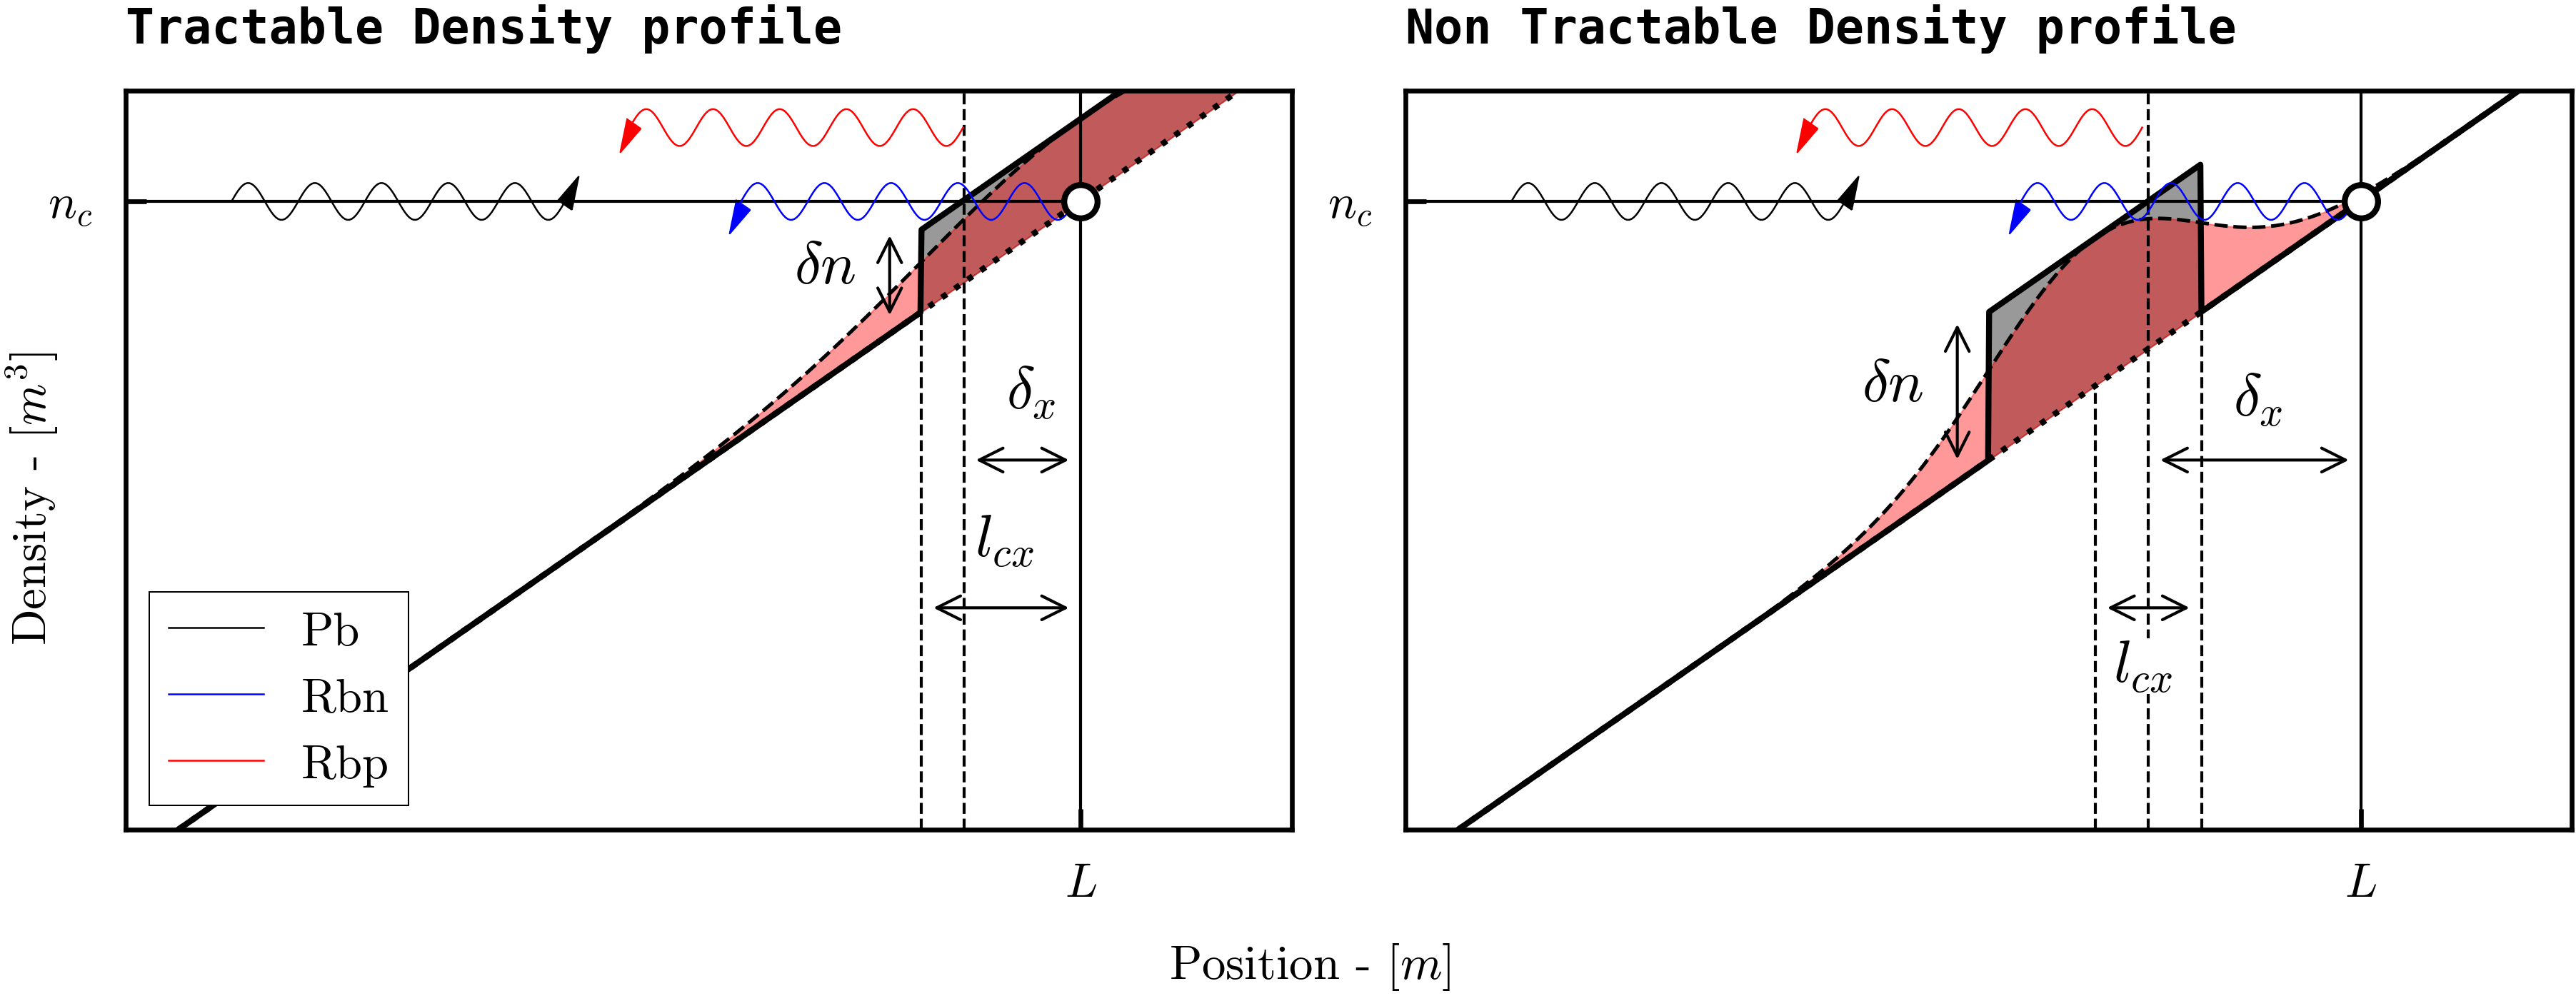
\includegraphics[width = 1\linewidth]{./figures/density_profile.png}
    \caption{Here we plot the density profile of the plasma for different perturbation amplitude, in grey the step-like model perturbation and in coral the gaussian one. For large value density perturbation, the model leads to a contradiction with its assumption $\delta x < l_{cx}$ or $\delta n < n_c \frac{l_{cx}}{L}$ , given by a small cut-off layer shift. The blue Pb wave is the probing wave, red Rbp wave is the reflected one and blue Rbn wave is the normal reflected wave, in absence of perturbation.}
    \label{Density_profile}
\end{figure}
\begin{multicols}{2}
    One sample of density fluctuation is produced using the following formula, to match a supposed gaussian spectra of instabilities :
    $$\delta n(k_x) = \delta n_0 \exp\left(-\frac{(kl_{cx})^2}{8} + i\Phi(k)\right)$$
    with $\Phi(k)$ a random phase, k the radial wavenumber of the density perturbation and $\delta n_0$ the amplitude of the perturbation, this amplitude can be taken constant or dependant of the radial position according to the kind of profile we use. Then we inverse fourrier transform this density perturbation to get the density profile in the real space. Finally, for each sample, the delay is then numerically integrated from the formula [cite delay], using simple trapezoidal integration.
    \paragraph{Results}

    The results are shown in the figure \ref{fig:std_delay}, the simulated deviation of delay (black cross) was computed on 10000 samples to ensure statisctial stability, with a 50 GHz probing wave and a $2L$ integration domain, allowing us to take into acccount negative perturbation near the cut-off, indeed if there is multiples ones near the standard cut-off it might strongly shift this latter. The plain black line is the 1st oder approximation of the formula [eq] and the dashed one as the third order approximation of the second focmula. The nuemarically integrated delay, which stands as reference is in black cross. The second order analytical formula presents a characteric drop-off (as the simulated delay) after reaching a critical value amplitude. This critical value can be defined by two way \cite{SPR_Krutkin, PUT} and fix the threshold of waht we could later the \textbf{Non linear} regime. Which can suggest than expanding further the $\sigma_{\tau_d}$ which leads to a better handling of non-linear domain. However, in both cases some discrepancies are observed for large perturbations in Non Linear regime, but the analytical expression seems to be a good approximation for small perturbations, except for really tiny one [cite]. However, One have to introduce a correction factor to the analytical expression to get a better agreement with the numerical integration. This $l_{cx}$ dependant factor is given has not been studied yet but it highlights the linitations of current step driven 1D model \footnote{The integration of the gaussian integral was also tackled, with a second order bell-approximation, leading to logarithmic dependancies over the plasma parameters, however the formula was to complicated to exhibits the statistical properties of the delay refers to appendix}. The non linear regime is strongly related to scattering effect, which are not taken into account in this approach. In addition to that, generally the density corrugation reachs a level of 100 \% of the density value near the cut-off \cite{Krutkin_thesis}, especially since the adiabatic and non adiabtic component of the electron response have the same potential dependancy \cite{San_diego}.   Hence the non-linear regime is non negligible and of necessity to find a sufficiently precise model to evaluate turbulences amplitudes in \textbf{NL} regime.

    \begin{figure}[H]
        \centering
        \hspace*{-1cm}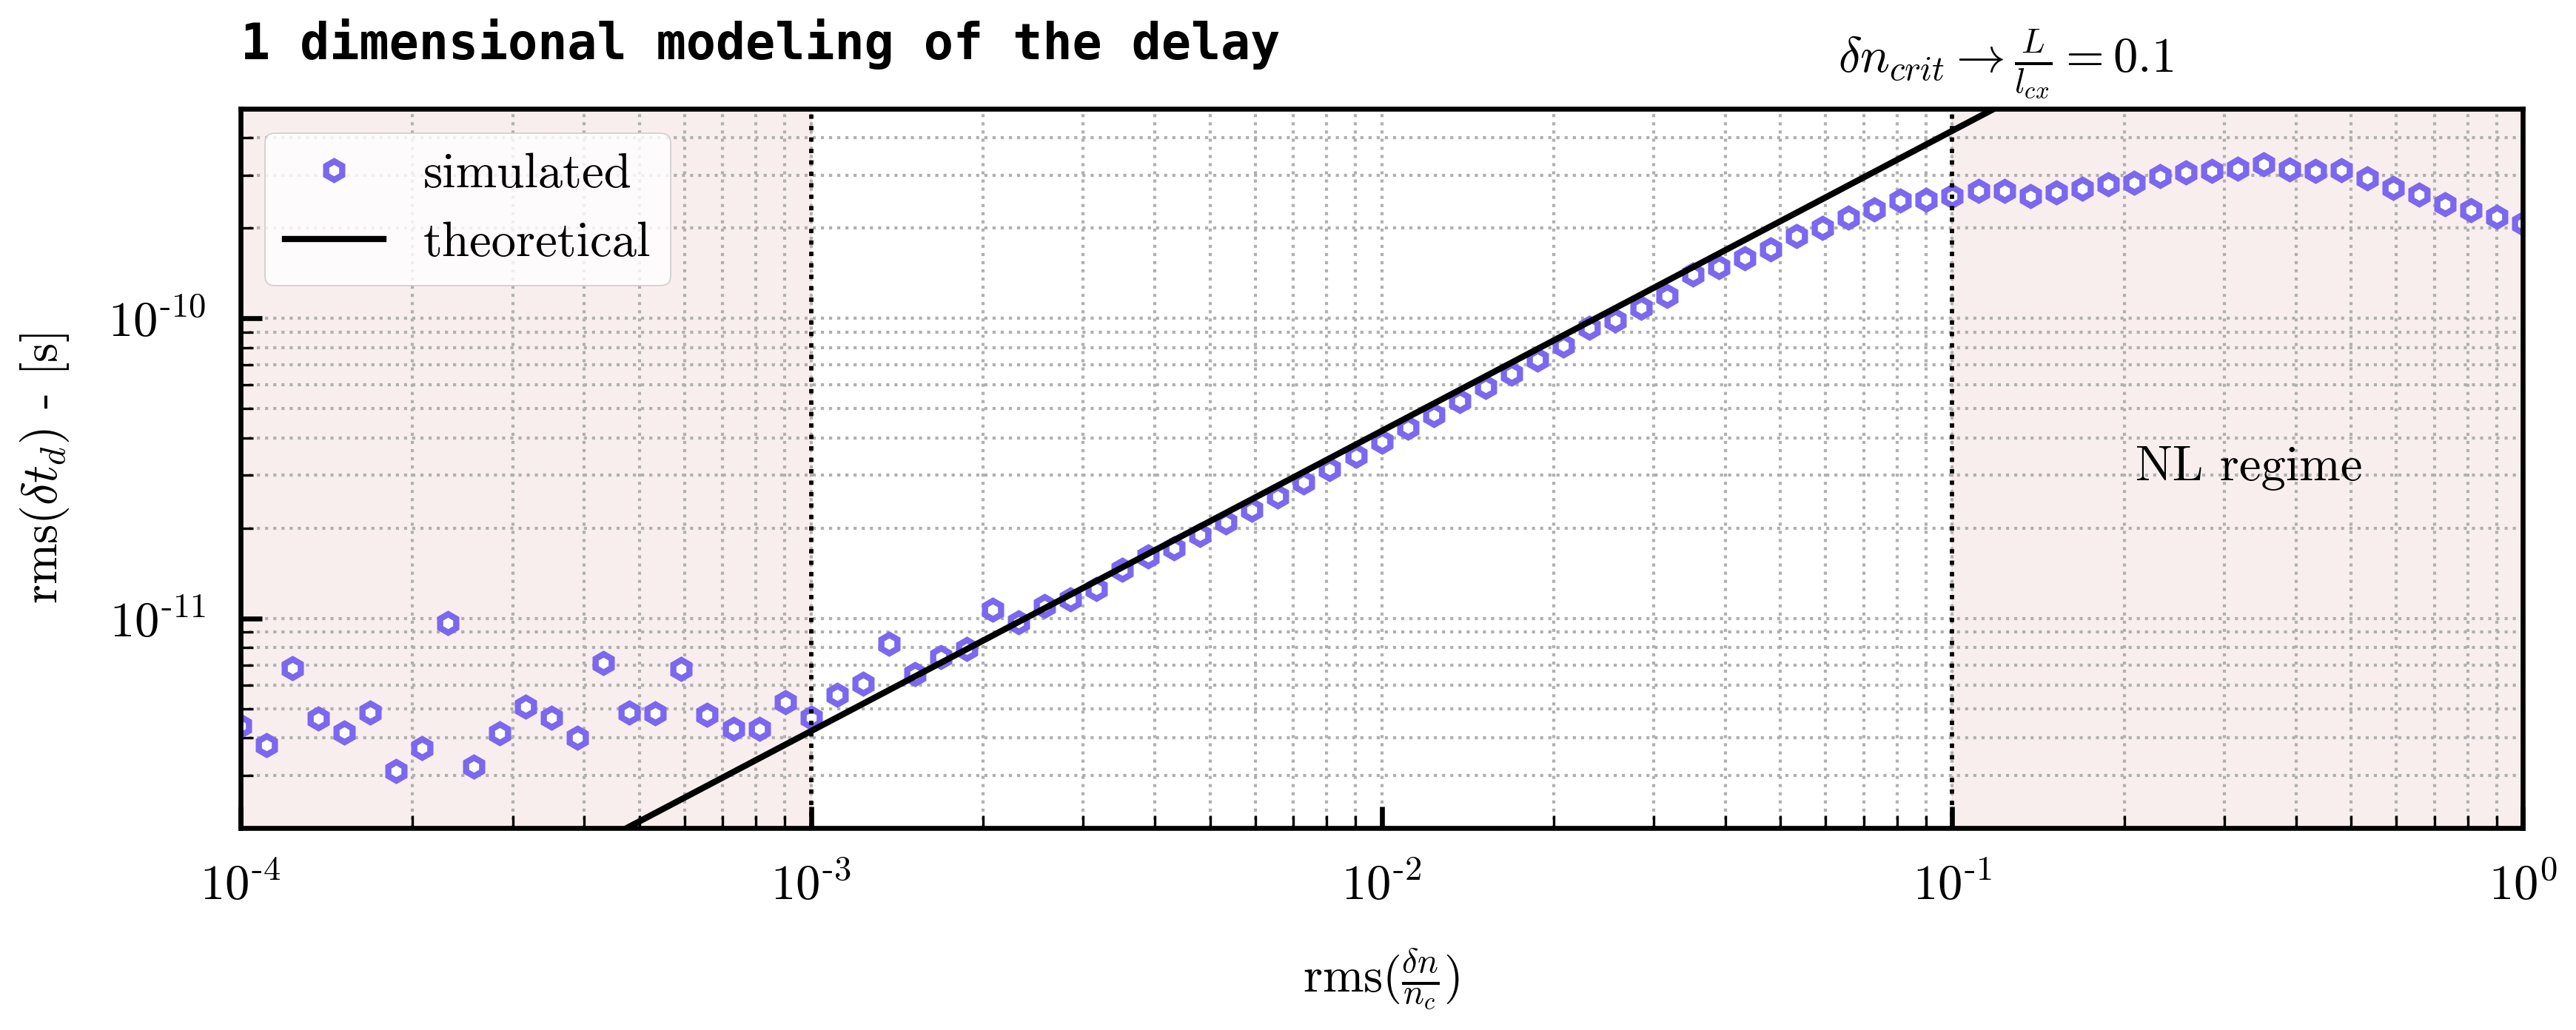
\includegraphics[width=1\linewidth]{./figures/1d.pdf}
        \caption{1 dimensional predicted amplitude of the analytical 1st and 2nd order step driven model, compared to the simulated 1 dimensional delay see eq :\ref{eq:Dispersion_relation}, a constant $\delta n_0$ has been used for the density profile}
        \label{fig:std_delay}
    \end{figure}
    Hence, the first arised issue is to find a good parametrization of the model (i.e find the best statisctial metrics) to predict the amplitude of the turbulence. This study will be done using several profile of density perturbations amplitudes $\delta n_0$, to see if the model we build is sufficiently robust to adpat.
    \chapter{1 dimensinal Model}
    The first model we tried to build relies simply on the 1 dimensional integration of the delay.
    Hence, for this simple model wa can only rely on the pulse delay statistical properties. Several options had been tested from the study of the quantile repartition of the delay, its histogram , and several statisctial properties of this latter. Then the study consists in a simple multi-dimensional regression problems where we will try to estimate the amplitude of the perturbation and the non-perturbed delay of the probing wave (i.e without the turbulenecs fields) and this for several density profile. In order to tackle this problem we used a stacked regressor, combined with a multi-output one.
    \section{Reliable metrics}

    To train our Machine Learning model, we need some clear data, with the best input as possible. So first let's try to understand the characteric of the delay. To have a general overview of the influence of the turbulence amplitude $\delta n_0$ on the delay characteric, the best way is to study the distribution of this latter in function of the amplitude, this is done in the following plot.

    \begin{figure}[H]
        \centering
        \includegraphics[width=1\linewidth]{figures/delay_overview.pdf}
        \caption{Violins plot of the delay distribution over $\delta n_0$, Here we choose for a simple first apporach a simple linear profile with $\delta n_0$ independant of the radial position. The left side of each violins stands for the 2d distribution of the delay for comparison.}
        \label{fig:Violins_delay}
    \end{figure}
    The first thing that we can unearth is that the delay distribution is well disturbed by an amplitude increasing, the mean delay decrease (which is quite obvious see \ref{fig:Density_profile}), the standard deviation of the delay increases and when we reached the non-linear regime it starts decreasing. The distribution seems also to be more more skewed until we reach the non linear regime, this indicates that the study of the momemt of the delay distribution can also be a good way to predict the amplitude level. The two-simulation sets present quite the same behaviour, however at high amplitude the 1d simulation set present some discrepancies with the 2d one, indeed the distribution is more eratic, this can question the good convergence of the 1D integration (see : \ref{eq:Dispersion_relation}). In addition to that, we can highlitht that the critical density unearthed by this plot is the first critical density (CITE), which is of great importance to buiiold a qualitiative dataset. Still, the delay study should lead to a good estimation for both simulation sets, even without pulse shapes study allow with the 2D model.
    Hence, let's see if the delay study can be a sufficient estimator for amplitude level prediction in both dimensionalities.

    \section{Machine Learning Model}
    The machine Learning model will learn to predict the amplitude $\delta n_0 $ and the default delay without amplitude $\tau_0 $ , with one one dimensional training set, and will be test on a one dimensional and a two dimensional testing set.
    \subsection{structure}

    The regression model we used is a stacked-multioutput regressor, it combines the following models : K-neighbors (\texttt{KNN}), Random-forest (\texttt{RF}), 3 different Gradient-Boosting (\texttt{GB}, \texttt{LGBM}, \texttt{XGB}), and support vector (\texttt{SVR}) , regressors, it is made to be as general and versatile as possible. Then the 6 models are trained in parallel on the same training datasets, in series with a decision regression model which is in our case a final \texttt{RF} layer trained on the outputs of previous layers.T

    Normally the Gradient-Boosting models can not handle multi-output regression, this is why we used a multi-output \href{https://scikit-learn.org/stable/modules/generated/sklearn.multioutput.RegressorChain.html}{\texttt{RegressorChain}}. This model train the model to predict the the first entry and then to predict the second given the first prediction, this allows to incorporate a dependancy between the different outputs, which should not be the case here, so normally a simple \texttt{MultiOutputRegressor} should be sufficient. Let's note that the score of the final model cannot be less than the score of the best model. The following table described the hyperparameters used for the stacked model.

    \begin{table}[H]
        \centering
        \begin{tabular}{||c | c||}
            \hline
            \textbf{Model} & \textbf{Hyperparameters}                                                                                    \\
            \hline\hline
            \texttt{KNN}   & \begin{tabular}[c]{@{}c@{}}\texttt{n\_neighbors} : 20 \\ \end{tabular}                                      \\
            \hline
            \texttt{RF}    & \begin{tabular}[c]{@{}c@{}}\texttt{n\_estimators} : 300\\ \texttt{max\_depth} : 40\end{tabular}             \\
            \hline

            \texttt{GB}    & \begin{tabular}[c]{@{}c@{}}\texttt{n\_estimators} : 200\\ \texttt{lr} : 0.005\end{tabular}                  \\
            \hline

            \texttt{LGBM}  & \begin{tabular}[c]{@{}c@{}}\texttt{n\_estimators} : 200\\ \texttt{lr} : 0.005\end{tabular}                  \\
            \hline

            \texttt{XGB}   & \begin{tabular}[c]{@{}c@{}}\texttt{n\_estimators} : 200\\ \texttt{lr} : 0.005\end{tabular}                  \\
            \hline

            \texttt{SVR}   & \begin{tabular}[c]{@{}c@{}}\texttt{kernel} : 'rbf'\\ \texttt{C} : 1 \\ \texttt{epsilon} : 0.01\end{tabular} \\
            \hline
        \end{tabular}

    \end{table}
    \captionof{table}{Main Hyperparameters used for the stacked model, the error use is not detailed as long as the performance tweaks}

    \section{Input Data}


    \section{Datasets building}


    For the 1D based trained model, we can only use the delay distribution as input variables. We tried several moment of the distribution as input (mean, variance, skewness...), combined with the discrtized delay distribution. We tested two types of discretization, the binned distribution and the quantile distribution. However, we reached better results with the quantile study of the distribution, coupled with the moments as input. This allows the model to have a direct connection between the output $\tau_0$ and the quantilized distribution. We use in both case 30 quantiles to discrtized the distribution. The 1D simulations set is then processed, splitted in a training and a testing set (80/20 ratio) and finally standardized, the amplitude parameter was used with its logarithmic value because it was find to be more efficient. Hence we arrived to a final input shape of 33 features and $\sim$ 3000 samples, including the $L$, $l_{cx}$ paraemters in the input data. For the 1D simulation, we introduced a random shift in the delay distribution for each sample, indeed if we dont do that the model will learn $\tau_0$ value from the highly coerrelated paraneter $L$ (originally $L$ is linear with $\tau_0$  ) which might be not the case in experimental data, where $L$ can stand for the gradient scale at the cut-off \cite{Krutkin_thesis}. For this study we used several density profiles to see if they have a real impact on the learning process of the model. For the 1D simulations the dependancy over $y$ is dropped.
    For the linear background profile, the global density profile will be the following :
    $$n(x,y) = n_c \frac{x}{L} + \delta n_0(x) \delta n(x,y).$$ With $\delta n $ the 2D gaussian turbulence profile
    For the quadratic background profile L, stands for the gradient scale at the cut-off, and $\delta n_0$ the turbulence amplitude profile . Here we choose the following formula to get the value of 1 of the gradient at L, which gives us :
    $$n(x,y) = n_c \left[1.25 - \frac{(1.5L_0 - x)^2}{L_0^2} \right] + \delta n_0(x)\delta n (x,y)$$
    The negative values of the profiles are then shifted to zerosm to prevent unphysical event, which has the effet of making a bigger vaccum layer in the simulations.
    The dependancy of $\delta n_0$ will take severqal form, from constant to linear, quadractic or exponentially ponderated \cite{SPR_Krutkin}, this scaling of the turbulences is done to mimic the true turbulence profile (REF), and to avoid the non natural preponderance of turbulences while working with small amplitudes. This exploration of the density profile is motivated by the fact that at the edge of the plasma, the relative amplitude of the turbulence profile is higher than in the core of the plasma.

    For reproductibility the  parameters of the 1d simulation used to build the considerated datasets are given bellow: .
    \setlength{\tabcolsep}{.038\linewidth}
    \renewcommand{\arraystretch}{1.5}
    \begin{center}
        \begin{tabular}{ccccc}
            \toprule
            \multicolumn{5}{c}{Parameters range}                       \\
            \cmidrule{1 -5}
            $\delta n_0$   & $l_{cx}$ -[cm] & L -[cm]  & $N_x$ & n     \\
            \midrule
            $[1e^{-3}, 1]$ & $[0.1,1]$      & $[7,20]$ & 5000  & 10000 \\
            \bottomrule
        \end{tabular}
    \end{center}
    \section{Results}
    A goos way to evaluate the model is to study the residuals of this latter for each parameters value of the testing set. It allows to have a quick overview of the performance model, and on the impact of parameter value on the model performances.

    \begin{figure}[H]
        \includegraphics[width=0.98\linewidth]{./figures/polar_param_1d.pdf}
        \caption{Plot of the amplitude residuals of the model for the 1D testing set in Non linear regime, the residuals are meaned given a value of the studied simulation's parameter. The filled curved stands for the amplitude residuals exponentially rescaled to the real amplitude value, The red line in the center of the plot is the $\tau_0$ mean residuals, far bellow the mean amplitude residuals. The second smaller polar shows the comparison of the residuals for several daasetets : the plot of the mean amplitude residuals for the 2D datasets (black dashed curve), the amplitude residuals for the 1D datasets (blue curve in the center), and the plots of the residuals for the 2D datasets shifted to the 1D delay distribution (green curve).}
        \label{fig:polar_1d}
    \end{figure}
    From this we reach a final score of 0.94 without the moment and 0.96 with the moments on the 1d test datasets. However, with  the 2d datasets the results appear to be catastrophics. The model generally predict an amplitude level one odm bellow or higher than the real one

    The figure \ref{fig:polar_1d} unearths quite good results regarding the 1D model prediction for the 1D testing simulation datasets, the predicted is generally of the same order of magnitude than the real one, and the residuals are quite well distributed among all the simulation parameters which is quite comforting. However, when we try to generalize the model to a higher dimension, here 2D simulations we reached very bad results with a mean amplitude residuals value of 10 for any simulations parameters. This can be explained by the fact that 1D simulations does not take into account multiple scattering effect when we reach non linear regime (see \ref{eq:Dispersion_relation}), however we can note that in non-linear regime on the 1D tetsing simulation datasets the model is far more performant than the analytic one. However, one can question the fact that the delay distribution is similar betweeen the 2D case and the 1D case. Indeed, for the same 1D parameter, we can find a shift between the mean value of the delay for the 2D simulations sets and the 1D simulations set, this is due to the layer of void added around the computation domain in the 2d simulations \cite{SPR_Krutkin}, and also because the pulse is not launched at $t=0$. Then, if we shift the 2D simulation delay datasets to the 1D simulations delay (which is of course questionable), we reach quite a good score even in non-linear regime (this observation as been done with a flat 2D geometry, and does not take into account crucial 2D simulation parameters as the probing angle or the curved profile), the residuals obtained is the order of 2 times the value of the amplitude which is relatively good kmowing the logarithmic scale of the amplitude during the training process.

    However, one can ask if the study of the pulse shape with different of its characterics can lead to better results. Indeed it will akkiw to take into account the multiple scattering effect, and the dispersive effect of the plasma. This will be the subject of the next chapter.
    \chapter{2 dimensinal Model}
    Considering a 2 dimensional model allows us to take int o account several interesting effect that plays a great role in the \textbf{SPR} diagnostic. Indeed, the 1D model restricted the study to delay distribution. With the CUWA 2D simulations, in addition to the delay we can study the pulse shape and its statistical properties. Furthermore, this added dimesion support the curvature $\frac{1}{R}$ study which is implies by the tokamak geometry. We can also tweak the probing wave incidence angle $\theta$, we will study the impact of these new model's parameters on the model performances, and see if the introduction of mmore complexity in the model can lead to better results, with the 2d simulations datasets.
    \section{Pulse shape Study}
    The goal of the pulse shape study is to find the best metrics that carry the more informations as possible, in order to make our model lighter and more efficient.
    \subsection{Relative Study of Pulse Shape}

    For this part of the study we will limit ourselves to a simple slab geometry with normal probing, without considering any curvature and incident angleThe pulse shape can give us some information about the plasma density profile, since the pulse shape can be modified by the presence of perturbations due to multiple scattering effects and dispersive effects [see \ref{eq:Dispersion_relation}].
    The dependance of the pulse shape over the background density profile will be also studied with linear, quadratic and linear modified perturbation profile. One can expect to have a much larger and randomness dependent pulse, at high turbulence amplitude due to multiple scattering. Indeed the reflected pulse will be a superposition of all scattered pulse, which should be characterized by a growing tail of the pulse distribution in delay and in width
    \begin{figure}[H]
        \centering
        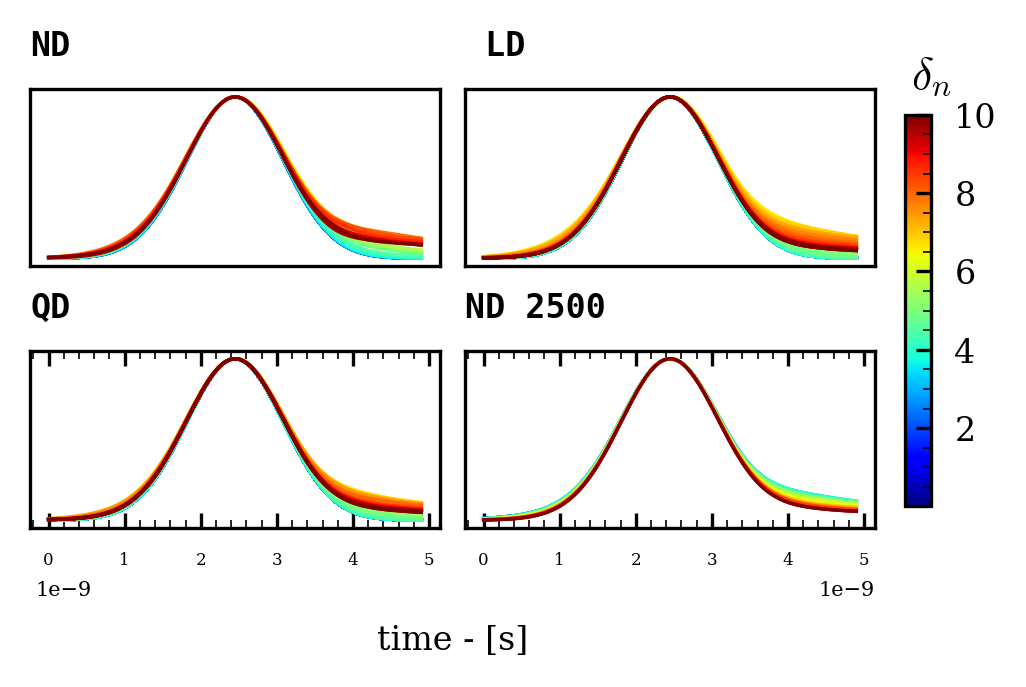
\includegraphics[width=1\linewidth]{./figures/pulse_shape.png}
        \caption{Nornalized Mean of reflected pulse signal, for several density profile \textbf{ND} stands for linear density profile with a linear dependancy of $\delta n_0$ over $x$  , \textbf{LD} is a simple linear density profile with a constant turbulence amplitude, \textbf{QD} is the quadratic density profile, \textbf{ND 2500} is a 2500 samples simulations (the amplitude range is no more respected for this one due to computation cost). }

        \label{fig:barrier}
    \end{figure}

    For all density profile, the pulse shape is getting broader and broader for large perturbations, and the delay is getting larger and larger. This is due to the presence of multiple scattering, and dispersive effects From this overview of the normalized mean pulse shape, we can see that a interesting metrics for our model should measured how much the mean pulse is skewed. This can be characterized by the study of the mean skewness of the pulse shape. (One other intersting paramter to highlithts is the hysteresis of the normalized mean pulse(i.e the ratio of the right area over the left area of the pulse).

    \begin{figure}[H]
        \centering
        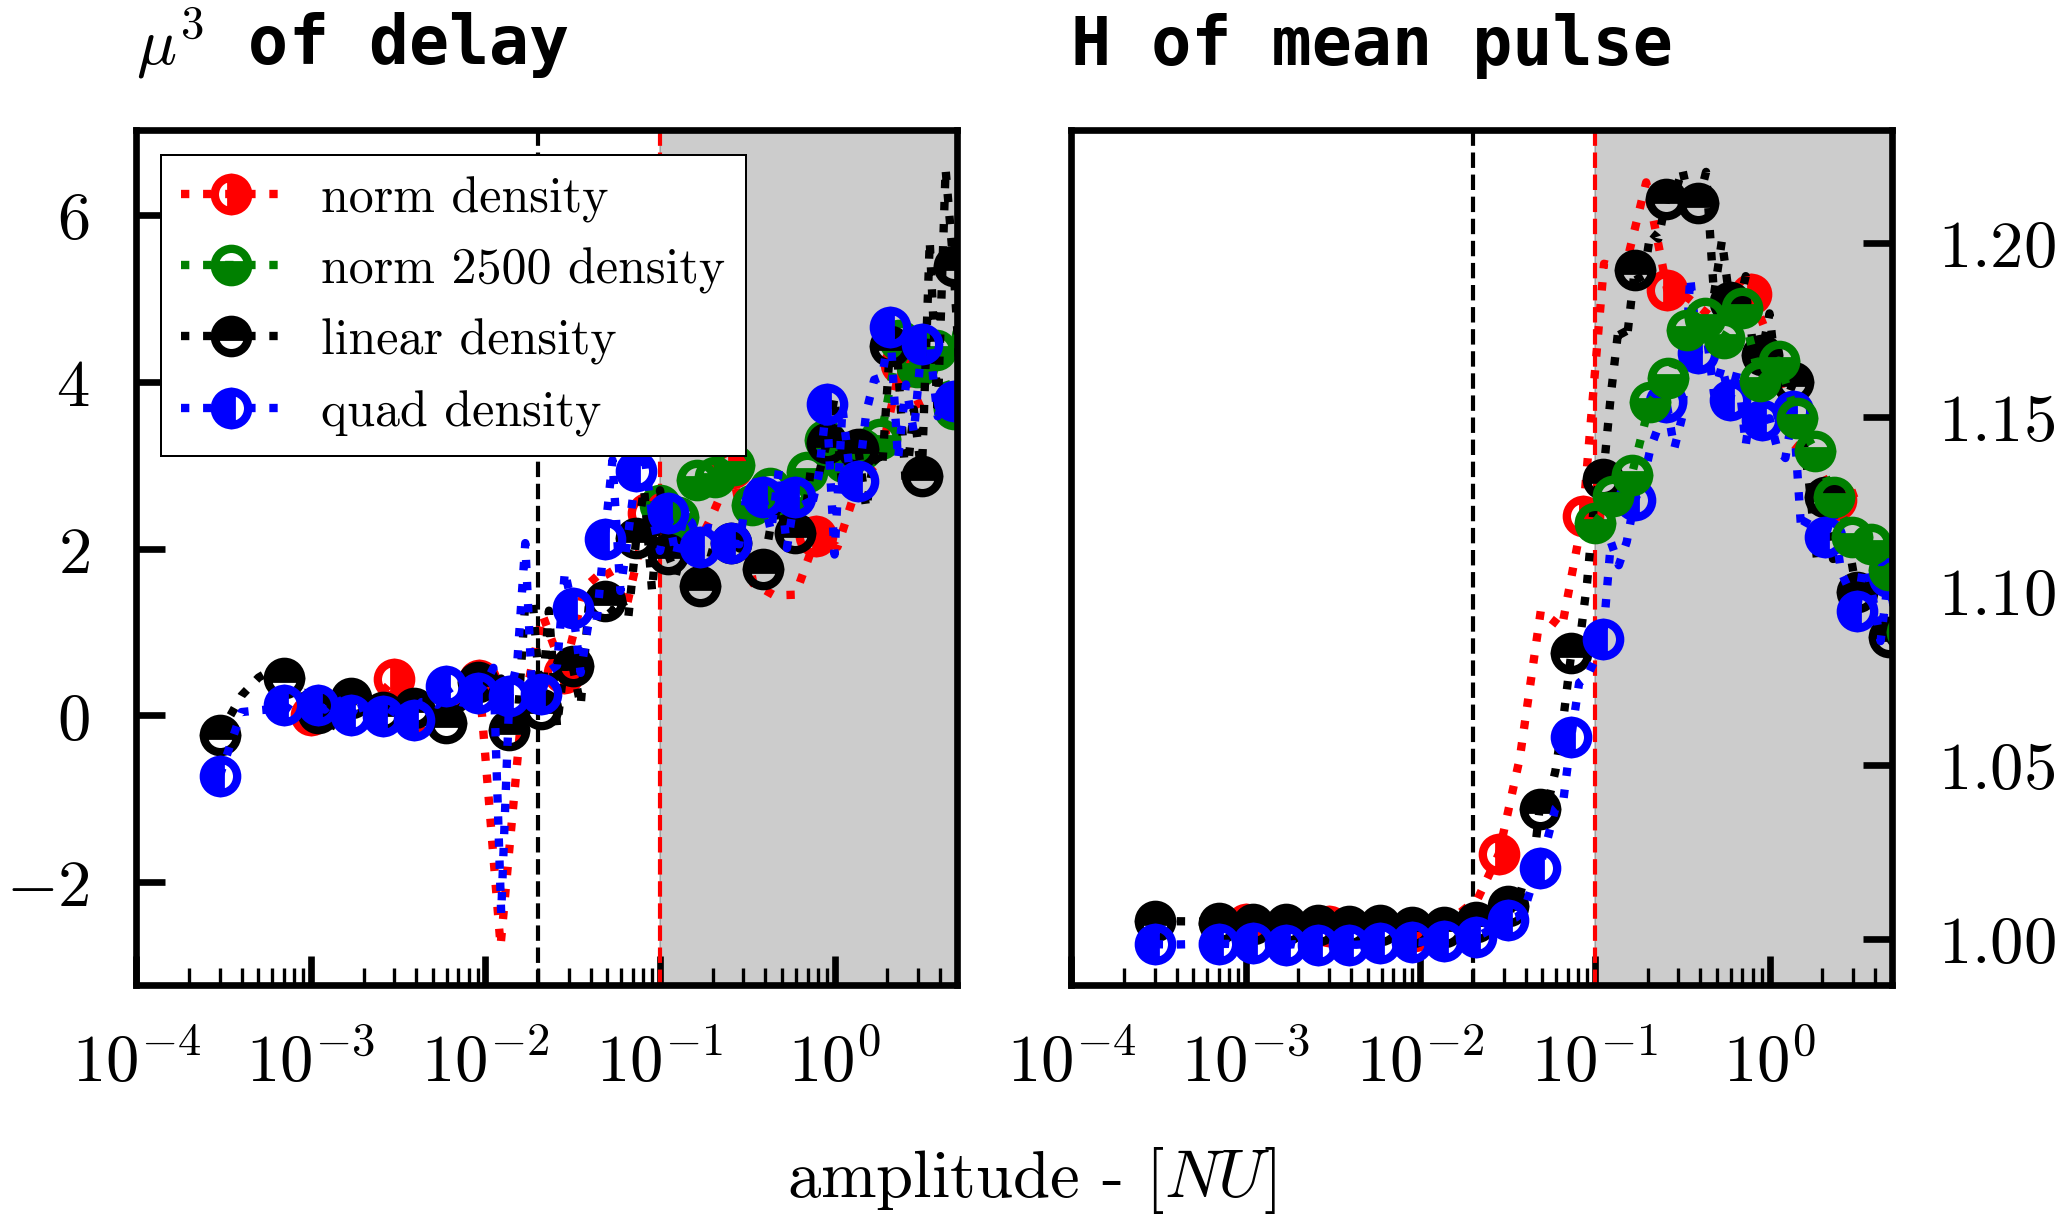
\includegraphics[width=1\linewidth]{./figures/skew_Hyst.png}
        \label{}
    \end{figure}

    \captionof{figure}{Here we computed the skewness $\mu^3$ and the hysteresis \textbf{H} of the mean pulse for the previous density profiles, as intended the skewness of the pulse is increasing, the hysteresis evolution is even more pronounced. One important thing to note, is that both of the metrics are governed by the second critical density value \ref{CRITICAL}, when multiple scatterings are non-negligeable.}

    The two last metricss seems to be relevant input variables two described the relative pulse shape evolution over the amplitude level. After studying the evolution of the normalized mean pulse shape, we can study the statistical properties of the pulse shape, in order to find some relevant metrics to consider for our model. Furthermore, it highlights that to build our Non-Linear regime dataset, we need to include in the amplitude range both critical values, because they defined important variations respectively in the delay distribution and in the pulse shape characterics.
    \subsection{Statistical Study of Pulse Shape}




    \begin{figure}[H]
        \centering
        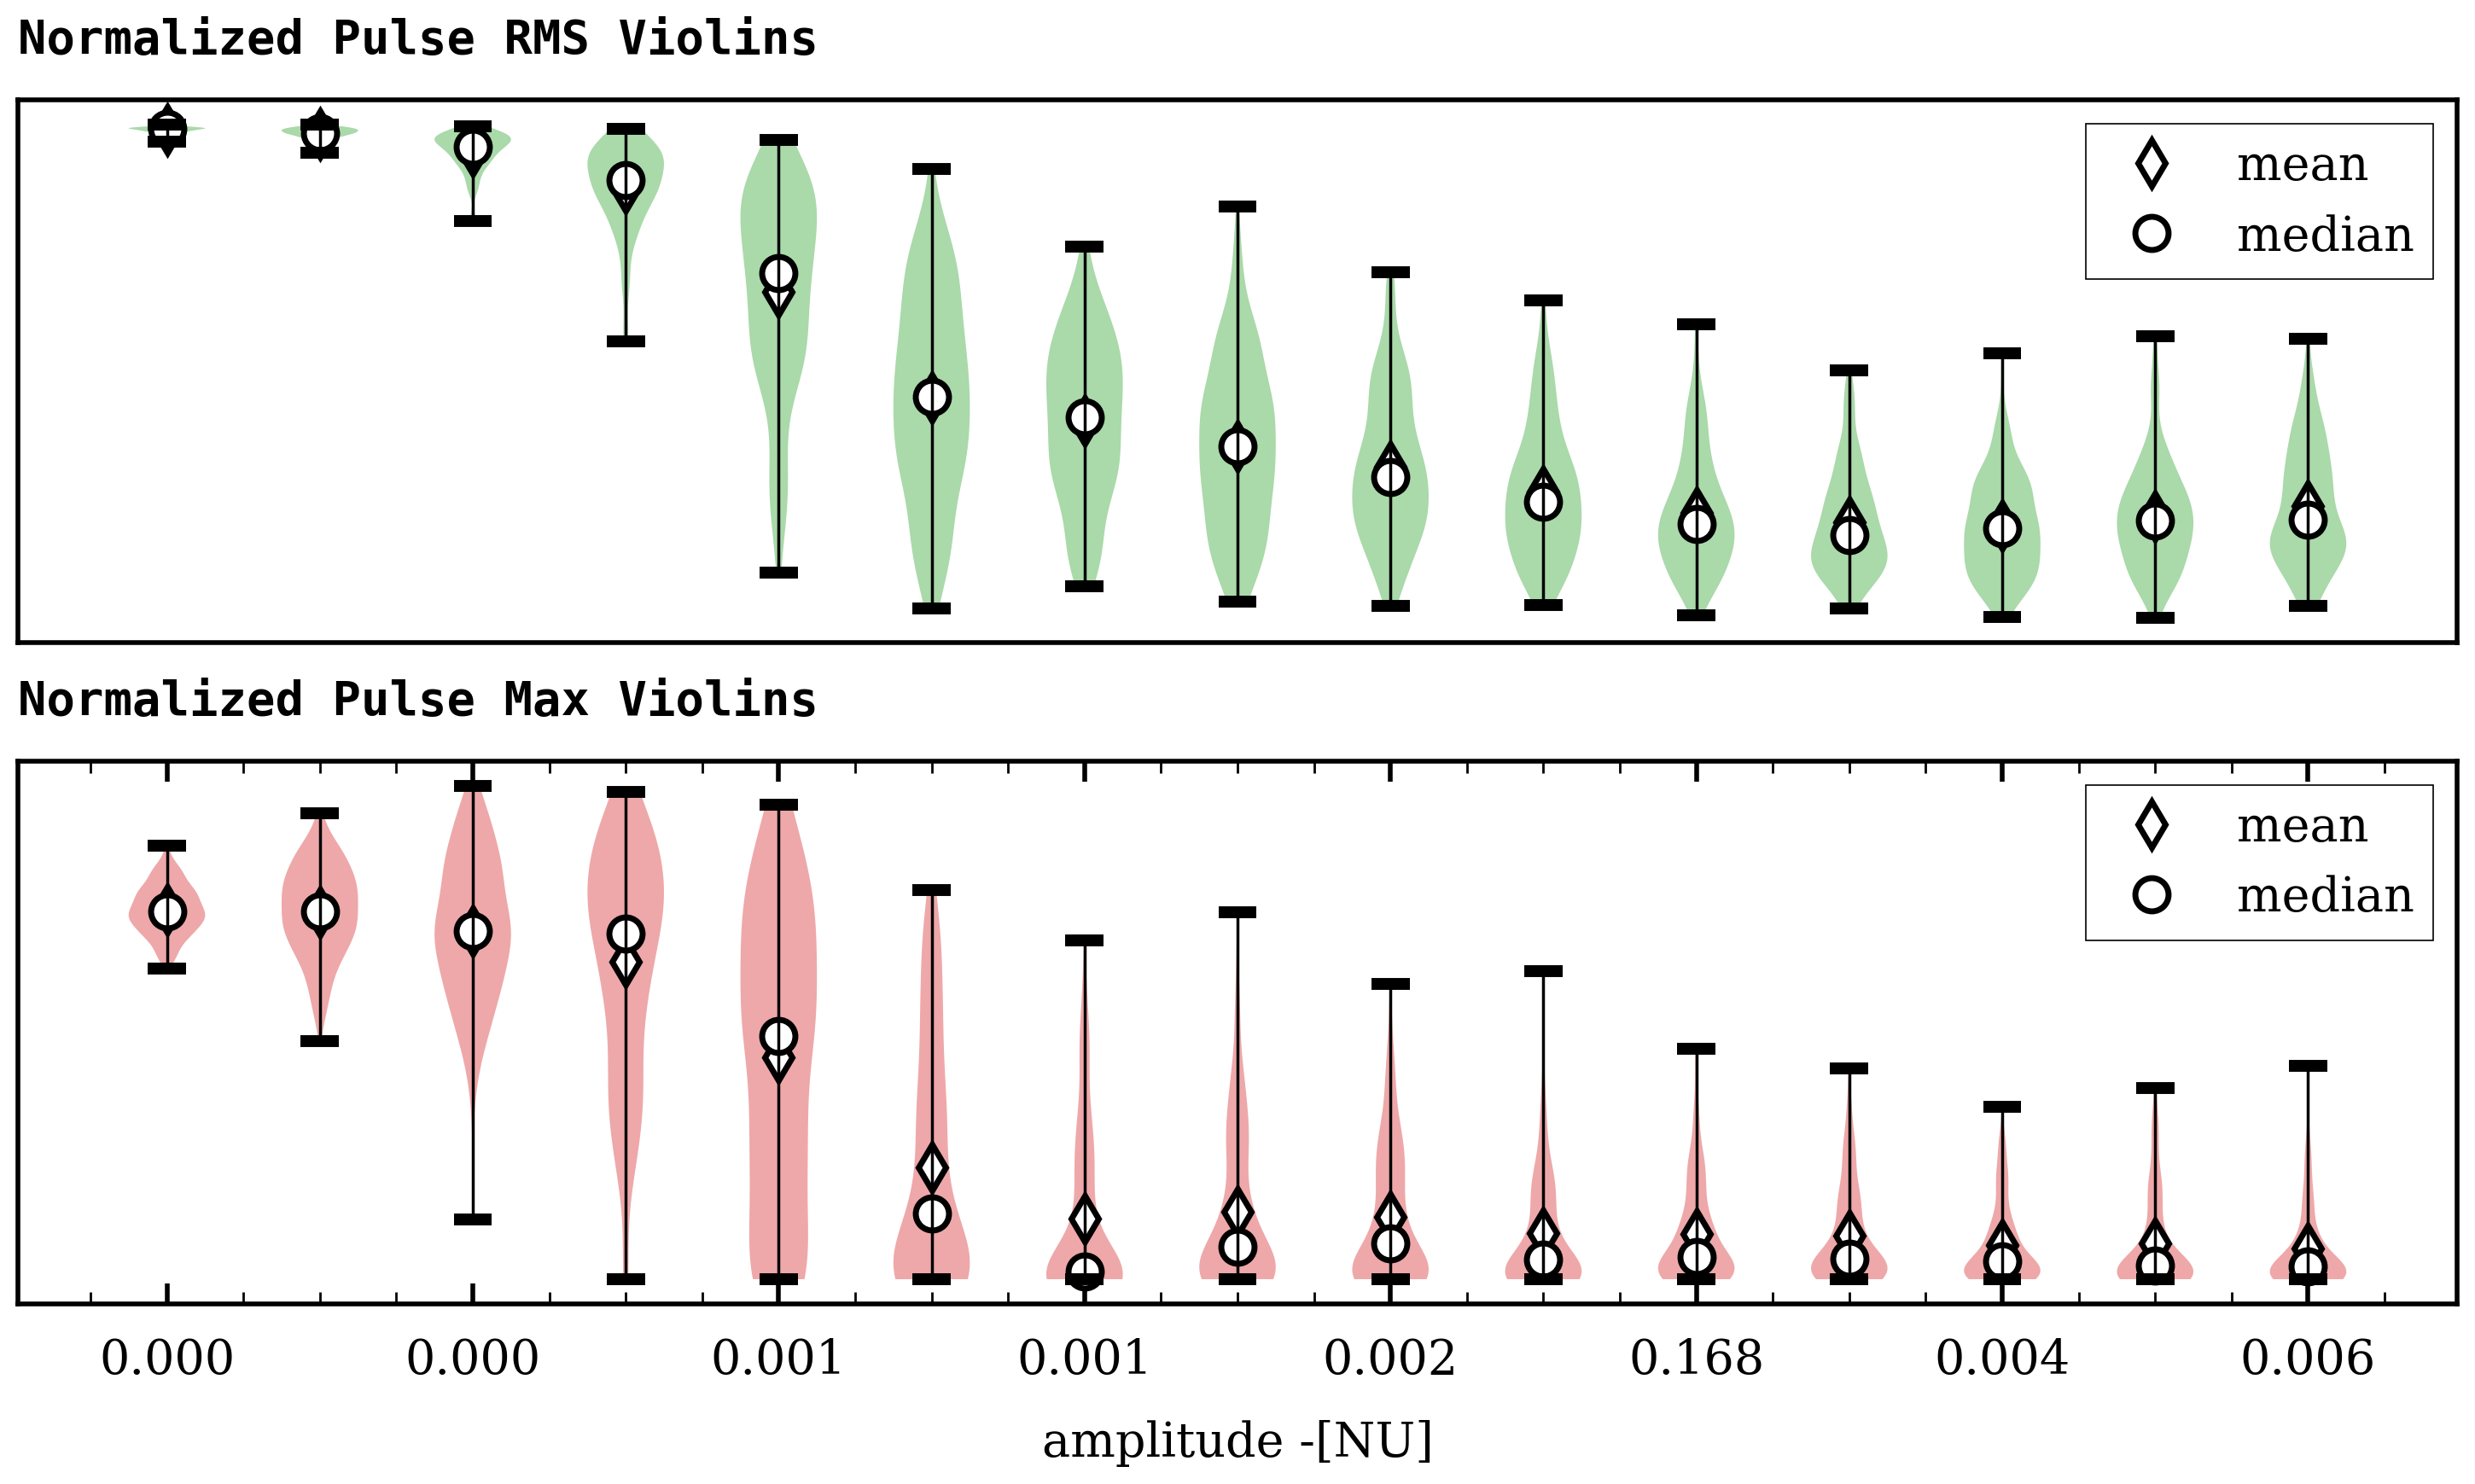
\includegraphics[width=1\linewidth]{./figures/pulse_overview.png}
        \caption{Here we plot the distribution of the pulse rms, amplitude and width for different perturbation amplitude, for the linear profile background profile \textbf{LD} . The distribution of the pulse rms  and amplutude is getting broader and broader during the transition regime, this is due to randomness introduced by the perturbations, which seems to remains at large amplitudes, even if the distribution is getting quite constant. Both amplitude and rms of the pulse are highly correlated seems to catch the same dependancy over the amplitude level and characterizes the transition regime between the two criotical densities. The pulse width distribution study seems to be more relevant in the Non linear regime with a very smooth evolution of the standard deviation and the maximum of the pulse width, we can note that the mean of the pulse with seems to be quite constant, and do not catch enough information to be studied.}
        \label{fig:barrier}
    \end{figure}

    From this study several conclusions can be drawn. First the mean of the pulse amplitude seems to catch enough information for the pulse amplitude distribution characterization. Secondly the pulse standard deviation evaluation is quite redondant with the amplitude study. And finally, the pulse wdith study throught the standard deviation of this latter can lead to interesting information, especially in full non-linear regime (after the second critical density). These conclusion have been drawn with a simple linear density profile,  we tested the two others density profiles (\textbf{ND}, \textbf{QD}), and it leads to the same tendancies. The only things we found, is a shift in the delay distribution due to the bigger vaccum layer when we use a quadratic density profile (see EQ)

    \subsection{Gaussian fitting of the pulse}
    On way to see the deformation of the gaussian pulse is to track the relative error of the gaussian pulse with a gaussian fit. Furthemore, it allows to study the true gaussian standard deviation, mean and amplitude.
    This is shown in the following figure, where we plot the relative error of the gaussian fit, and the gaussian fit
    \begin{figure}[H]
        \centering
        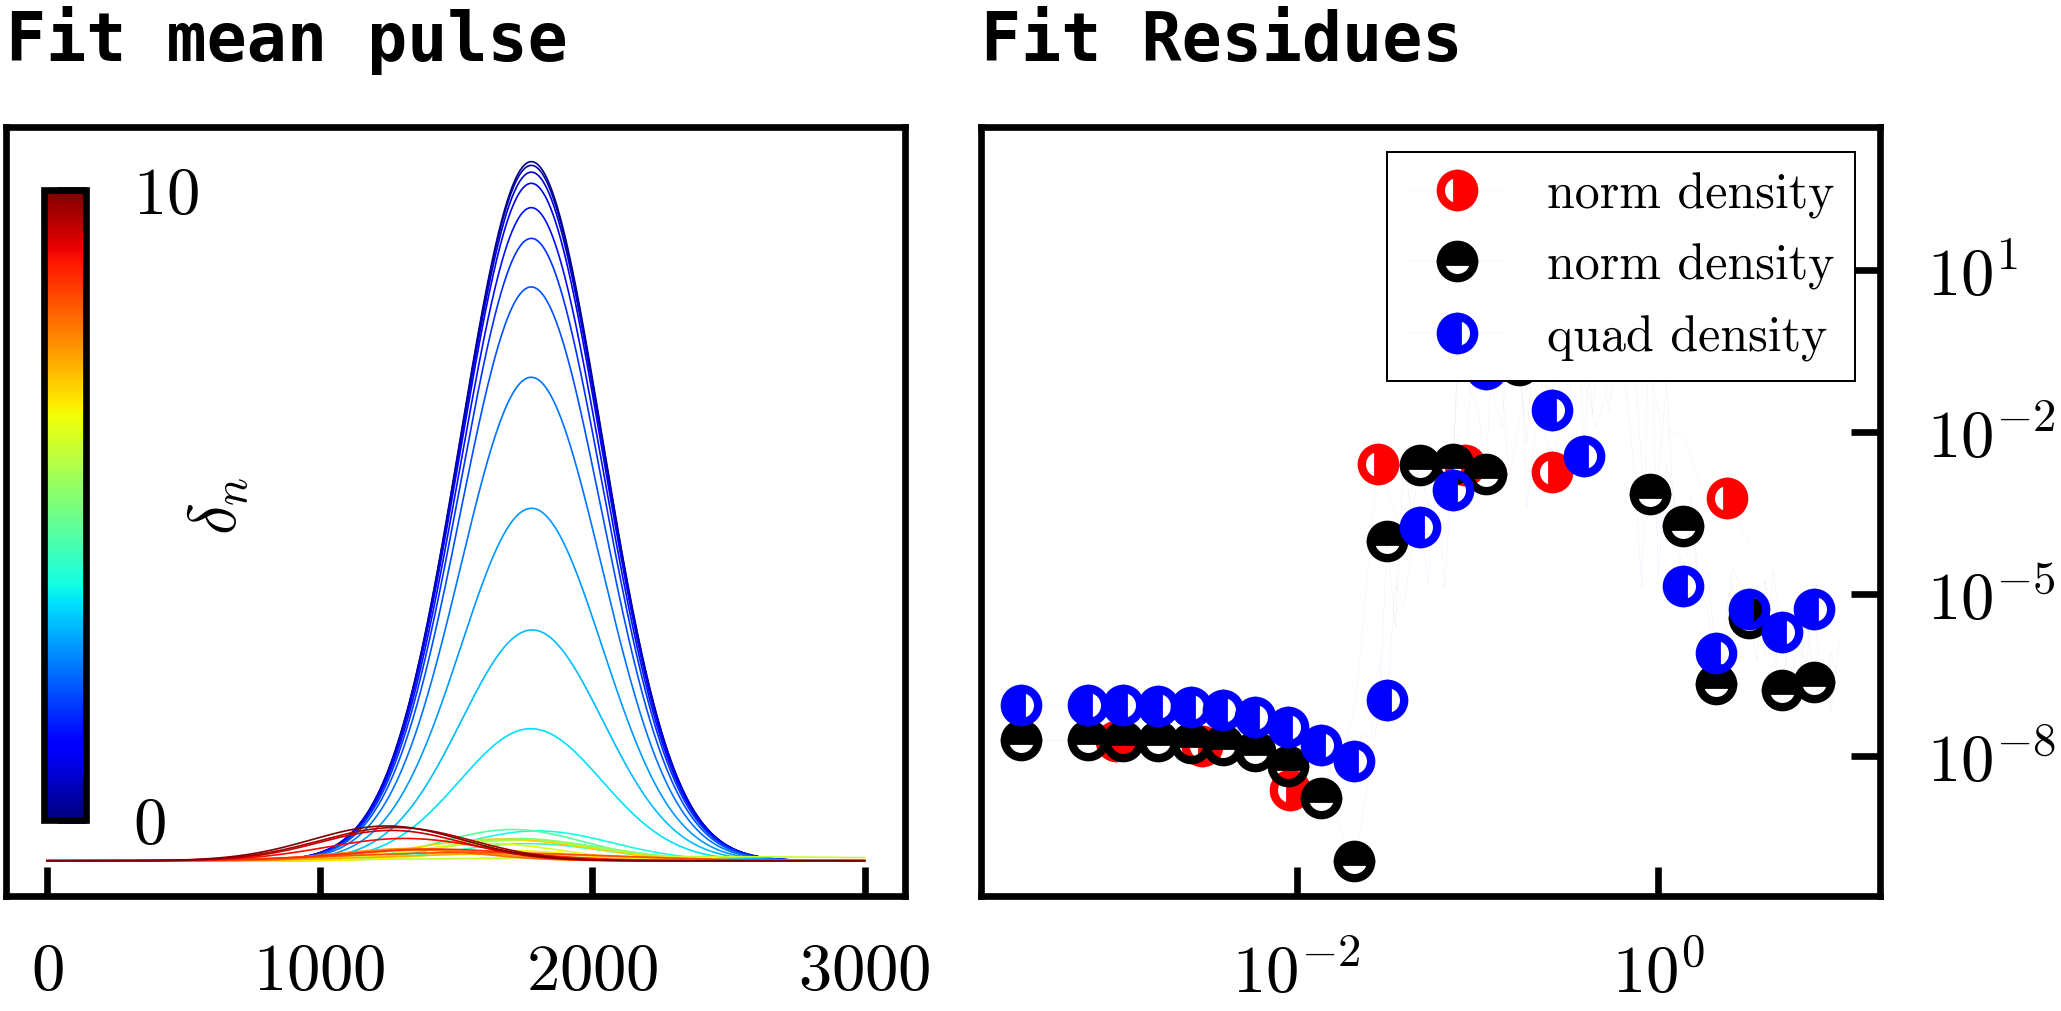
\includegraphics[width=1\linewidth]{./figures/gaussian_fit.png}
        \caption{The relative error of the Gaussian fit (residuals ponderated by the size of the respective pulse amplitude) is getting large for the transition zone of the pulse shape, and seems to decline for very large turbulence. However we have to find smooth metrics to characterize the transition, and not a pseudo-random one to have better predictions in the next part.
            The gaussian parameters are also good quandidates and are plotted in the next figure }
        \label{}
    \end{figure}

    \begin{figure}[H]
        \centering
        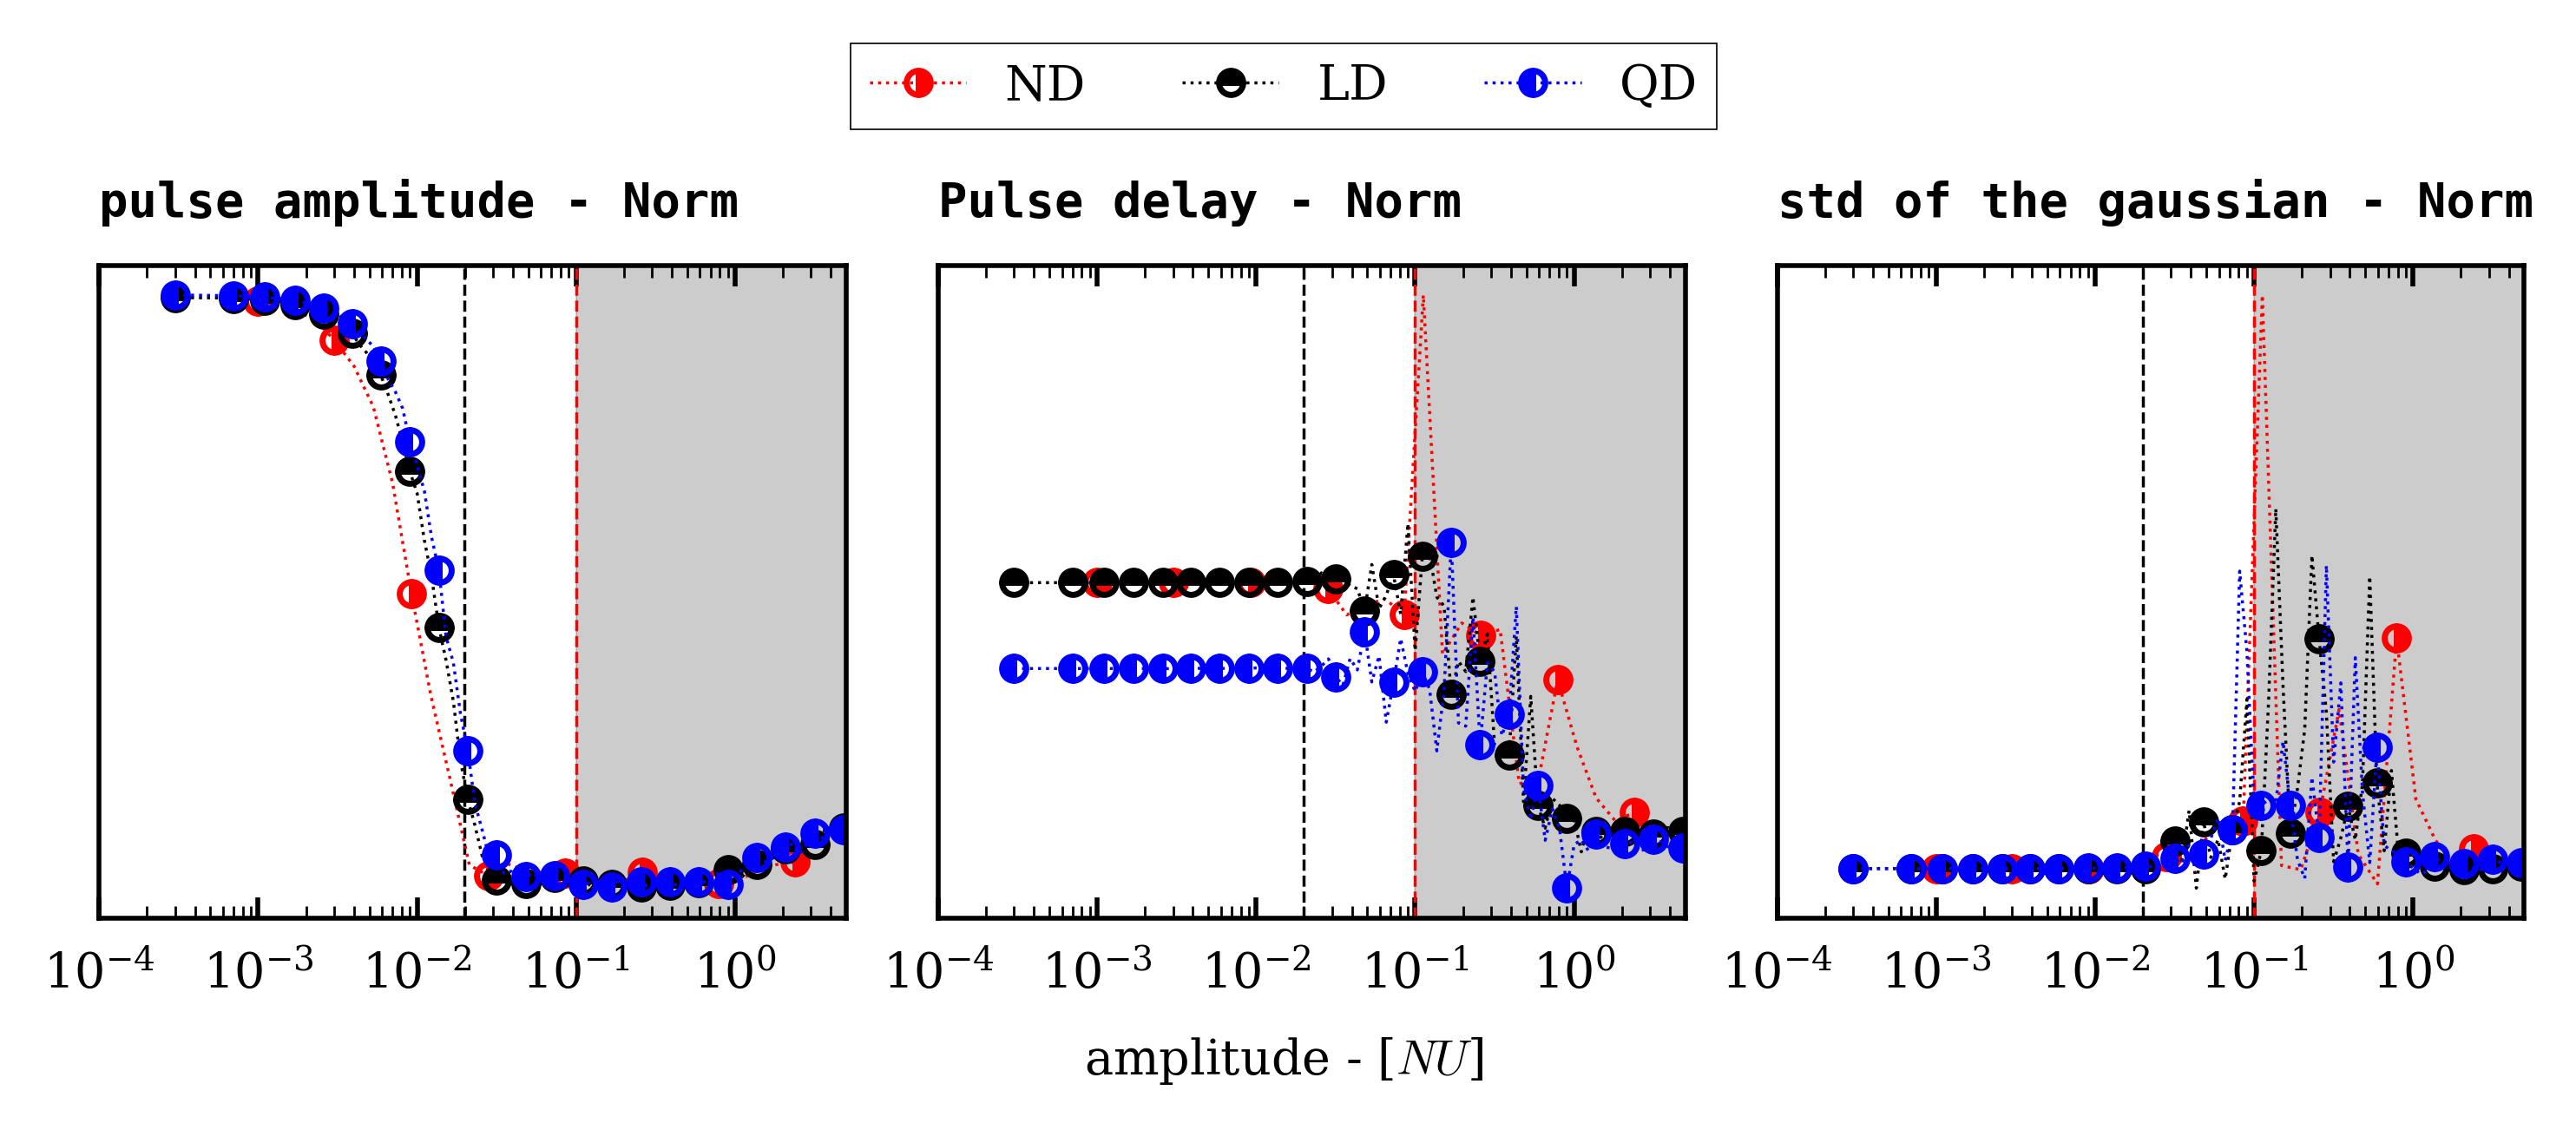
\includegraphics[width=1\linewidth]{./figures/gaussian_Params.pdf}
        \caption{Gaussian pulse delay and standard deviation have chaotic behavior during the transition regime, this made them not relevant candidate for the next study. However lets note that the gaussian pulse ampliutde,
            have quite a smooth behavior, but unearth a plateau during the non linear linear transition, which might not ne a good option, even if at large amplitude we capture the same behavior as for the non gaussian amplitude.
            In a much cleaner way, indeed it's clearly increasing, this might be interesting to study the highly non linear regime.}
        \label{}
    \end{figure}


    ADD SPIKE NUMBER

    \section{Datasets building}
    For the two dimensional datasets we select the following pulse metrics in addition to the quantilized delay distribution :  mean of pulse amplitude, standard deviation of delay, mean of Hysteresis, skewness of the mean pulse, standard deviation of pulse width.

    % - REDUCTION OF BM AND LCX CORR MATRIX
    % - PLOT WITH ALL THE CORR MATRIX
    % - USE SPIKEWIZARD
    % - LCy PARAMS FOR 2D with 1D COMPARISON
    % - 2D MODEL TRAINING
    % - 2D MODEL TESTING (AMP AND TD0)
    % - 2. Histogram of residual
    % - LEVERAGES
    \subsection{Gaussian spectrum of the turbulences}
    The gaussian spectrum is the most simple way to model the turbulence, and was used as first approximation to see if the model could integrate the dependancy of the diffrent correlation length. The parameter used for the 2D simulations with the CUWA code on \textbf{LEONARDO} are the following :
    \setlength{\tabcolsep}{.016\linewidth}
    \begin{center}
        \begin{tabular}{ccccc}
            \toprule
            \multicolumn{5}{c}{Parameters range}                                                \\
            \cmidrule{1 -5}
            $\delta n_0$   & $l_{cx}$ -[cm] & $l_{cy}$ -[cm]  & $\theta$ -[°] & $R$ -[m]        \\
            \midrule
            $[1e^{-3}, 1]$ & $\{1, 0.5 \}$  & $\{0.5,2,30 \}$ & [0-10]        & [0.2,5]\{1000\} \\
            \bottomrule
        \end{tabular}
    \end{center}
    $\theta$ stands for the incident angle of the probing beam, $R$ the geometry curvature, $l_{cx}$ the typical correlation length of the turbulence in the $x$ direction, and $l_{cy}$ the typical correlation length of the turbulence in the $y$ direction. The $R$ range is choosen to tackle flat and near TCV tokamak geometries, $\theta$ values are dependant of the $R$ range and cannot be to high, indeed if we consider a high curvature the incident angle cannot be too high, because the probing beam will not be able to reach the cut-off layer, or will be reflefed not in the direction of the antenna, this is why we limited ourselves to 10 degrees, with $R = 0.2$ m. In the gaussian case, the power spectrum of the turbulence arr given by the following formula :
    $$\delta n(\textbf{k} ) = \delta n_0 \exp\left(-\frac{(k_x l_{cx} k_y l_{cy})^2}{8} + i\Phi(\textbf{k} )\right)$$
    This formula will be used to create the first part of the dataset with defined correlation lengths. But one could argue that the power spectrum of \textbf{TEM} instabilities is not gauussian.
    \subsection{Power Spectrum of the turbulences}
    Indeed the power spectrum of the turbulences is a more realistic approach to the turbulence profile, (give the detail for each litterature measurements of the knee power spectrum). Then explain why the power spectrum is much more complicated to have a continuous one.
    Then introduce the formula of the power spectrum used [cite], and the different parameters used .
    $$<\delta n^2 > = \frac{1}{1 + \vert \frac{k_x}{W_x} \vert^\gamma + \vert \frac{k_y - k_y^*}{W_y}\vert^\beta}$$
    This formula has the advantage to not be separable in $x$ and $y$, which is the case in ... [cite]
    \begin{figure}[H]
        \centering
        \includegraphics[width=0.7\linewidth]{example-image}
        \caption{Power Spectrum and correlation length measurements, compared to the gaussian spectrum}
        \label{}
    \end{figure}

    \subsubsection{COrrelation length dependancy study}
    As it is not determied by the power spectrum formula we have to shift to measured lc as an input for the model. This is why its conveninent to have a relationship between all the parameters and the correlation length. The expression of lcx can be found using the Wiener-Khinchin theorem [], supposing $k_y$ constant fore the integration ::
    $$r_{x x}(\tau) = \int_{-\infty}^{\infty} <\delta n(k_x, k_y)^2> e^{2 \pi k_x \tau} \, dk_x$$
    With $r_{x x}$ the autocorellation function. The correlation length is then defined when the $r_{x x}$ reaches the $e^{-1}$ level, then developing the expression of the power spectrum, we have :

    \begin{align}
        r_{x x}(\tau) & = \int_{-\infty}^{\infty} \frac{1}{1 + \vert \frac{k_x}{W_x} \vert^\gamma + \vert \frac{k_y - k_y^*}{W_y}\vert^\beta} e^{2 \pi i k_x \tau} \, dk_x \\
                      & = \int_{-\infty}^{\infty} \frac{e^{2 \pi i k_x \tau}}{1 + \vert \frac{k_x}{W_x C^{1/ \gamma}} \vert^\gamma} \, dk_x
    \end{align}
    This expression is valid under the following limits\dots
    This leads to the following numerical expresion of the correlation length found fore the given paraameters of the power field,
    %     \begin{center}
    %         \begin{tabular}{ccccccc}
    %             \toprule
    %             \multicolumn{7}{c}{Parameters range}                                                                                                     \\
    %             \cmidrule{1 7}
    %             $k_y^*$                & $W_x$           & $W_y$                 & $\gamma$ & $\beta$ & $D$                                      & $ L$  \\
    %             \midrule
    %             $\frac{1e^{-4}}{\rho}$ & $frac{1}{\rho}$ & $frac{1e^{-4}}{\rho}$ & $4$      & $3.14$  & $6.3e^{-3}\left(\frac{\rho}{L}\right)^2$ & $0.1$ \\
    %             \bottomrule
    %         \end{tabular}
    %     \end{center}
    %     % \begin{cases}
    %     %     lc_x = 1.19402632 \rho + 0.00121852 \\
    %     %     lc_y = 1.35459058 \rho + 0.00152604
    %     % \end{cases}

    The real field is then obtain using the inverse fourier transform of the $\delta n(\textbf{k} )$ field. For each simulations we recorded the pulse signal with and without the turbulence field, and this for approximatively 500 samples. The raw data is then process online on LEONARDO to get the pulse metrics, and the delay distribution. This data is then saved in a SQL dataset build for this purpose and then trasnfer to the SPC computer for small data operations. We followed the same procedure as for the 1D dataset, with stantard normalisation, and same training/testing split, with the simulation parameters as input with the previous metrics and $\delta n_0, \, \tau_0$ as output.

    \subsection{data scanning}
    For the first part of the training to have homogeneous data distribution we chose data points on a defined grid, then to refined the model we used some random uniformly sample (logarithmicly for $\delta n_0$ ) data points in the range of the study.
\end{multicols}
\begin{figure}[H]
    \centering
    \includegraphics[width=1\linewidth]{./figures/polar_param.pdf}
    \caption{Polar distributions of the params}
    \label{}
\end{figure}

\begin{multicols}{2}
    \newpage
    \nocite{*}
    \printbibliography
\end{multicols}


\end{document}